\documentclass[10pt,a4paper,twocolumn]{jarticle}
\usepackage{graphicx}
\usepackage{bm}
\usepackage{amsmath}
\usepackage{booktabs}
\usepackage{das2022}%自律分散シンポジウム原稿用スタイルファイル

%Preamble
\pagestyle{empty}
%\mathindent0pt

\begin{document}

\twocolumn[
% 論文の和文題名
\begin{center}
{\Large \bf 画像認識ニューラルネットワークによる複数ロボットの対面走行}\\
%{\large \bf }\\
\vspace{2mm}
% 著者の和文名
{\large
     ○李 \ 方正(室蘭工業大学), 山田 \ 将司(室蘭工業大学),本田 \ 泰(室蘭工業大学)
}\\
\vspace{2mm}
% 論文の英文題名
{\Large \bf Bidirectional movements of multiple robots based on a neural network for image recognition}\\
%{\large \bf }\\
\vspace{2mm}
% 著者の英文名
{\large
     ○Li Fangzheng (Muroran Institute of Technology), Masashi Yamada (Muroran Institute of Technology),Yasushi Honda (Muroran Institute of Technology)
}\\
\end{center}

\vspace{1mm}
\baselineskip=1.0mm
{\small{\bf Abstract:} 

In previous research,we did some pseudo-ellipse course experiments of Face-to-Face movement with seasory motor mapping robots based on tanh function.
Then,we comfirmed the transference phenomenon from Face-to-Face movement to one-direction flow and measure the flow rate and time from start to one-direction flow.

In this paper, in order to shun one-direction flow, we made neural network model(input:960,middle:1000,output:2) which can analyse one-dimension image data and
did about five experiments of  neural network model and seasory motor mapping model in same course. 
From those experiments we know the robots can avoid obstacles smoothly and keep Face-to-Face movement for a long time successfuly.
Beside, we also proved the neural network model is better than seasory motor mapping model in robots flow rate, time of keep one-direction flow and turn around number through compare between two model.

 


}
\vspace{3mm}

{\small{\bf Keywords:} Swarm robot, Autonomous movement, Bidirectional movement , Neural network, 
Seasory motor mapping}

\vspace{5mm}

]
%}}

%%%% ベクトル用太文字の定義
%
%\newcommand{\bm}[1]{\mbox{\boldmath $ #1 $}}
%

\baselineskip=4.9mm%行間

\section{はじめに}
実世界で,蜂,アリなどの昆虫が簡単な行動メカニズムによって,複雑な群れ行為がよく観察される.
また,大きな交差点などにおいて,人間は密度が高くても,会話なしで,
ぶつからないようにスムーズに対面歩行ができる.
我々は,走行ロボットを使って,様々な自律走行アルゴリズムで対面走行実験を行って,
その対面走行など,自己組織化のメカニズムを解明することに目指す.

先行研究\cite{li}では,我々は双曲線関数により,
距離センサとモーターの出力が直接関連する感覚運動写像(省略名:SMM)ロボットを使って,
擬楕円コースで8台のロボットの対面走行の実験を行った.
結果として,コース幅の増加に従って,流量が増加して,
コース幅が56cmから安定になると確認した.
初期配置と初期向きを問わず,一定時間結果後,
すべてのロボットが同じ方向になって,1方向走行流が観察された.
理由として,距離データで向きを判断できないと考えている.
それに,3つの距離データで障害物の数を認識できず,
渋滞が起こることの原因になると考える.

本研究では,長時間対面走行ができ,流量を増やせるようにするため,
カメラを使って,中間層1層のニューラルネットワーク(省略名:NN)により1次元画像認識アルゴリズムを開発した.
コースに色をつけ,感覚運動写像とニューラルネットワーク2種類のアルゴリズムでコース幅1mの8台ロボットの対面走行を実験した.

結果として,ラジコンする時,ソースコード上曲がる値を拡大,
直接後退機能をつければ,ニューラルネットワークより自律走行性能が向上するとしった.
一方,方向転換のことをロボットに教えてないまま,1方向走行流になりにくく,感覚運動写像より,
ニューラルネットワークの方が壁や障害物(他のロボット)をスムーズに避けることができると観察した,流量も1.5になると確認した.


\section{ロボットの身体性}
今回使っているのはラズパイで制御する4輪走行ロボットである(Fig.\ref{robot_img}),
人間や昆虫の走行特徴に近似するため,その場で曲がり,方向転換が可能である.
ロボットの頭にカメラ(D)をつけていて,入力データを収集する.
E,Fは左右のモーター,独自で左右の車輪を制御して,ロボットを動かす.
A,B,Cは右,中央,左の距離センサーであり,感覚運動写像において用いる\cite{li2020}.
ロボット幅は13.5cm.長さは20.2cm.高さは12.2cmである.

\vspace{-4mm}
\begin{figure}[htb]
    \centering
    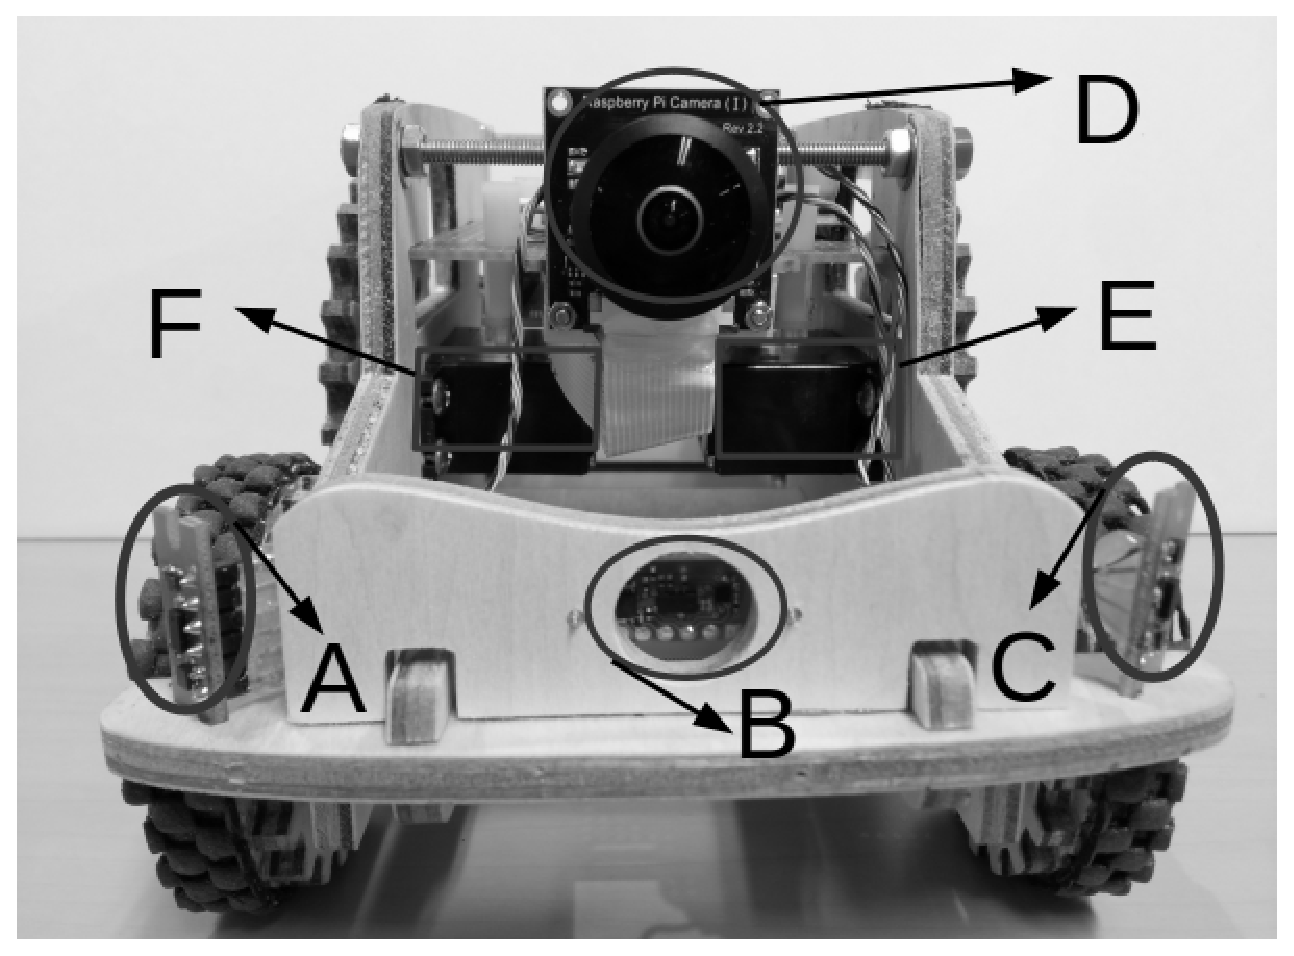
\includegraphics[width=0.4\linewidth]{robot1.eps}
  \label{robot_img}
    \caption{ロボット正面図}
\end{figure}





\section{ニューラルネットワーク}
\subsection{教師データの収集}
本研究では,
二次元画像データ(RGB)のピクセル値を縦方向($y$方向)にすべて足し合わせて一次元画像をつくる.
それらを並べたものを1次元画像ベクトル$\vec{u}$とする(\ref{eq:onedimension}式参照).

具体的に記述する.
カメラで撮影するのは$320 \times 240$のサイズのピクセル値であるが,不要な部分を切り取って,
130行目から200行目を切り出す.
コースの壁や障害物となる走行ロボット以外が撮影されている上下の部分を不要な部分とみなす.
つまりコース以外とロボット自身が映ってる部分をトリミングする(Fig.\ref{roboteye}参照).



その画像データのRed,Green,Blueそれぞれのピクセル値を要素としてもつ数値行列を
$\boldsymbol R,\boldsymbol G,\boldsymbol B$とする.
下記のように1次元画像$\vec{u}$を作成する.

\vspace{-2mm}
\begin{eqnarray}
\left\{
\begin{aligned}
\vec u_{\rm R}= \sum_{y=130}^{200} \boldsymbol R_{y}\\
\vec u_{\rm G}= \sum_{y=130}^{200} \boldsymbol G_{y}\\
\vec u_{\rm B}= \sum_{y=130}^{200} \boldsymbol B_{y}\\
\vec u = (\vec u_{\rm R}, \vec u_{\rm G}, \vec u_{\rm B}) \\
\end{aligned}
\right.
\label{eq:onedimension}
\end{eqnarray}
ただし,$\boldsymbol R_y, \boldsymbol G_y, \boldsymbol B_y$は
それぞれ$\boldsymbol R, \boldsymbol G, \boldsymbol B$の第$y$行だけを取り出したベクトルである.
$\vec u$は$960$列のベクトルとなる.

\begin{figure}[h]
\centering
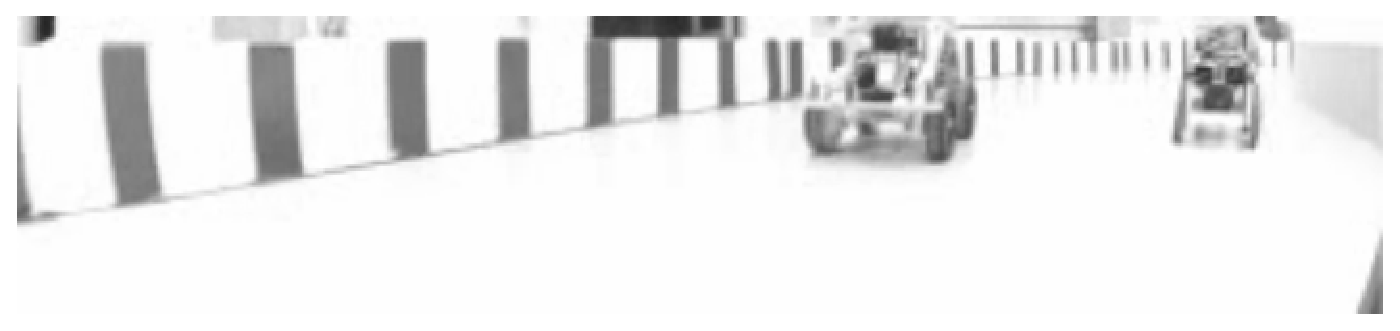
\includegraphics[width=0.7\linewidth]{robot_eye.eps}
\caption{ロボットの視点からのカメラ画像例}
\label{roboteye}
\end{figure}


\subsubsection{大きいハンドルで教師データ収集}
教師データは,コースに障害物(他のロボット,Fig.\ref{data_colle}の黒い円で囲まれてないロボット)をコースの中にランダムに置いて,
データ収集ロボットを手動操縦(ラジコン)して,
障害物と壁を避けながら時計回りと反時計回り両方走行して,教師データ収集する.
障害物の位置もランダムに変更して,合計3000個教師データ収集した.

\vspace{-2mm}
\begin{figure}[h]
        \centering
        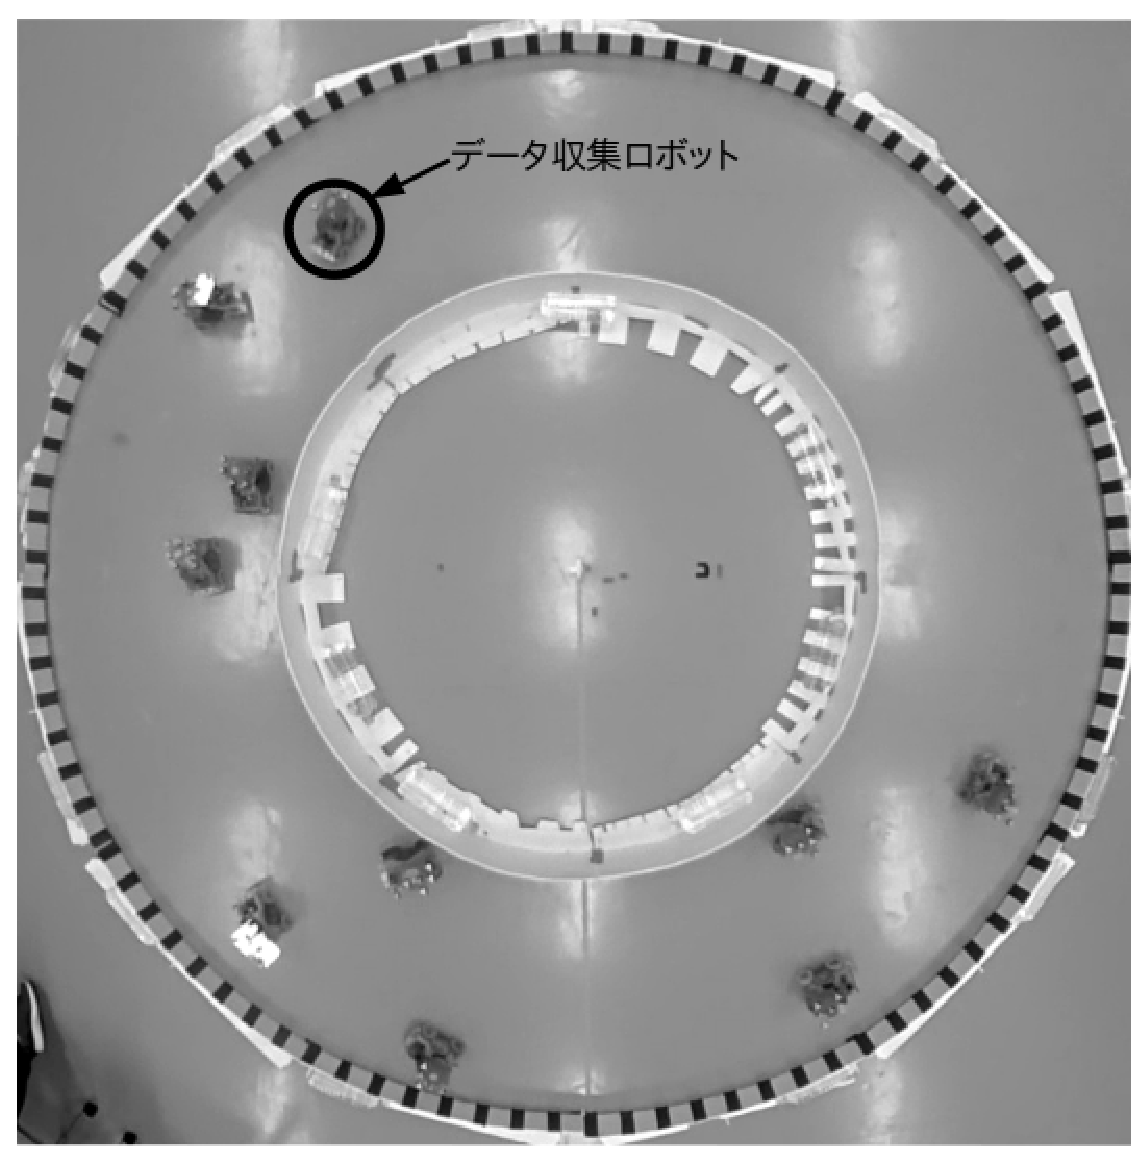
\includegraphics[width=0.8\linewidth]{teacher_collection.eps}
        \caption{円形サーキット}
        \label{data_colle}
\end{figure}

ラジコンの方法はTable.\ref{radio_rule}の大きいハンドルの部分を参照して,
"D"以外のボタンを押す瞬間の画像データを一次元画像データに変更して,
ソケット通信で学習用パソコンに送信して,教師データの収集を行う.
大きいハンドルというのは,ボタン"J"と"L"押すと,
モーターの出力が35単位変えるということである.

\begin{table}[!ht]
\caption{
大きいハンドルと小さいハンドルの違い
\label{radio_rule}}
\setlength\tabcolsep{1pt}
\begin{center}
\begin{tabular}{|c|c|c|c|c|}
\hline
 & \multicolumn{2}{|c|}{小さいハンドル} & \multicolumn{2}{c|}{大きいハンドル}\\
\hline
 操作& Left motor & Right motor & Left motor & Right motor \\
\hline
W & +20 & +20 & +35 & +35\\
\hline
S & -15 & -15 & -35 & -35\\
\hline
A & * & * & -56 & -56\\
\hline
D & * & * & =0 & =0 \\
\hline
J & -15 & +15 & -0 & +35 \\
\hline
L & +15 & -15 & +35 & -0 \\
\hline
K & \multicolumn{4}{|c|}{操作JとKで変化した出力が0になる} \\
\hline
\end{tabular}
\end{center}
\end{table}


\subsubsection{小さいハンドルで教師データ収集}
小さいハンドルで教師データ収集は大きいハンドルで教師データ収集と同じコースで収集する
,障害物については,止まってるロボット約6台,感覚運動写像より走行するロボット1台,
別の人がラジコンするロボット2台の環境で,データ収集ロボットをラジコンして,
障害物と壁を避けながら時計回りと反時計回り両方走行して,教師データ収集する.
合計6000個教師データ収集した.

ラジコンの方法はTable.\ref{radio_rule}の小さいハンドルの部分を参照して,
ボタンを押す瞬間の画像データを一次元画像データに変更して,
ソケット通信で学習用パソコンに送信して,教師データの収集を行う.
小さいハンドルというのは,ボタン"J"と"L"押すと,モーターの出力が15単位変えるということである.


\subsection{データの学習}
入力層のニューロン数は960(一次元画像データの値の数)とした.
中間層のニューロンの数を100から1100まで変更して,学習を行った.
Fig.\ref{anti_left}の横軸は中間層ニューロンの数,
縦軸は左のモーターの予測出力と教師データ出力の平均二乗誤差である.
Fig.\ref{anti_right}の横軸は中間層ニューロンの数,
縦軸は右のモーターの予測出力と教師データ出力の平均二乗誤差である.
中間層のニューロンの数の増加に従って,回帰誤差の増減に規則性はみられない.
経験によって,中間層のニューロンの数を1000にした.

左右のモーターの制御パワーを計算するので,出力層ニューロンの数を2にする.
活性化関数としてrelu関数を用いた.

最適化アルゴリズムとしてAdamでバッチ学習を用いた.

Adamのパラメーターとして
$\alpha$=0.01,$\eta$=0.3,$\beta$1=0.9,$\beta$2=0.9,$\epsilon$=$1\times e^{-8}$.$w$=0
を用いた.

Fig.\ref{LeftOutput}とFig.\ref{rightOutput}は学習終わったニューラルネットワークの
回帰結果部分的グラフである.
横軸はデータの番号(1番目から600番目の教師データをグラフした),
縦軸は左のモーターの出力(Fig.\ref{LeftOutput})と右のモーターの出力(Fig.\ref{rightOutput})である.
%オレンジ色の線が教師データの出力で,青色線が教師データと同じの入力(1次元画像データ)でニューラルネットワークの予測出力です.
ニューラルネットワークの予測出力が教師データの出力に完璧に回帰していないと見られるが,
人間のラジコンで収集した教師データも完璧ではないと考えて,ある程度回帰できれば,実際の走行実験の振舞いで評価を行う.

\vspace{-2mm}
\begin{figure}[h]
        \centering
        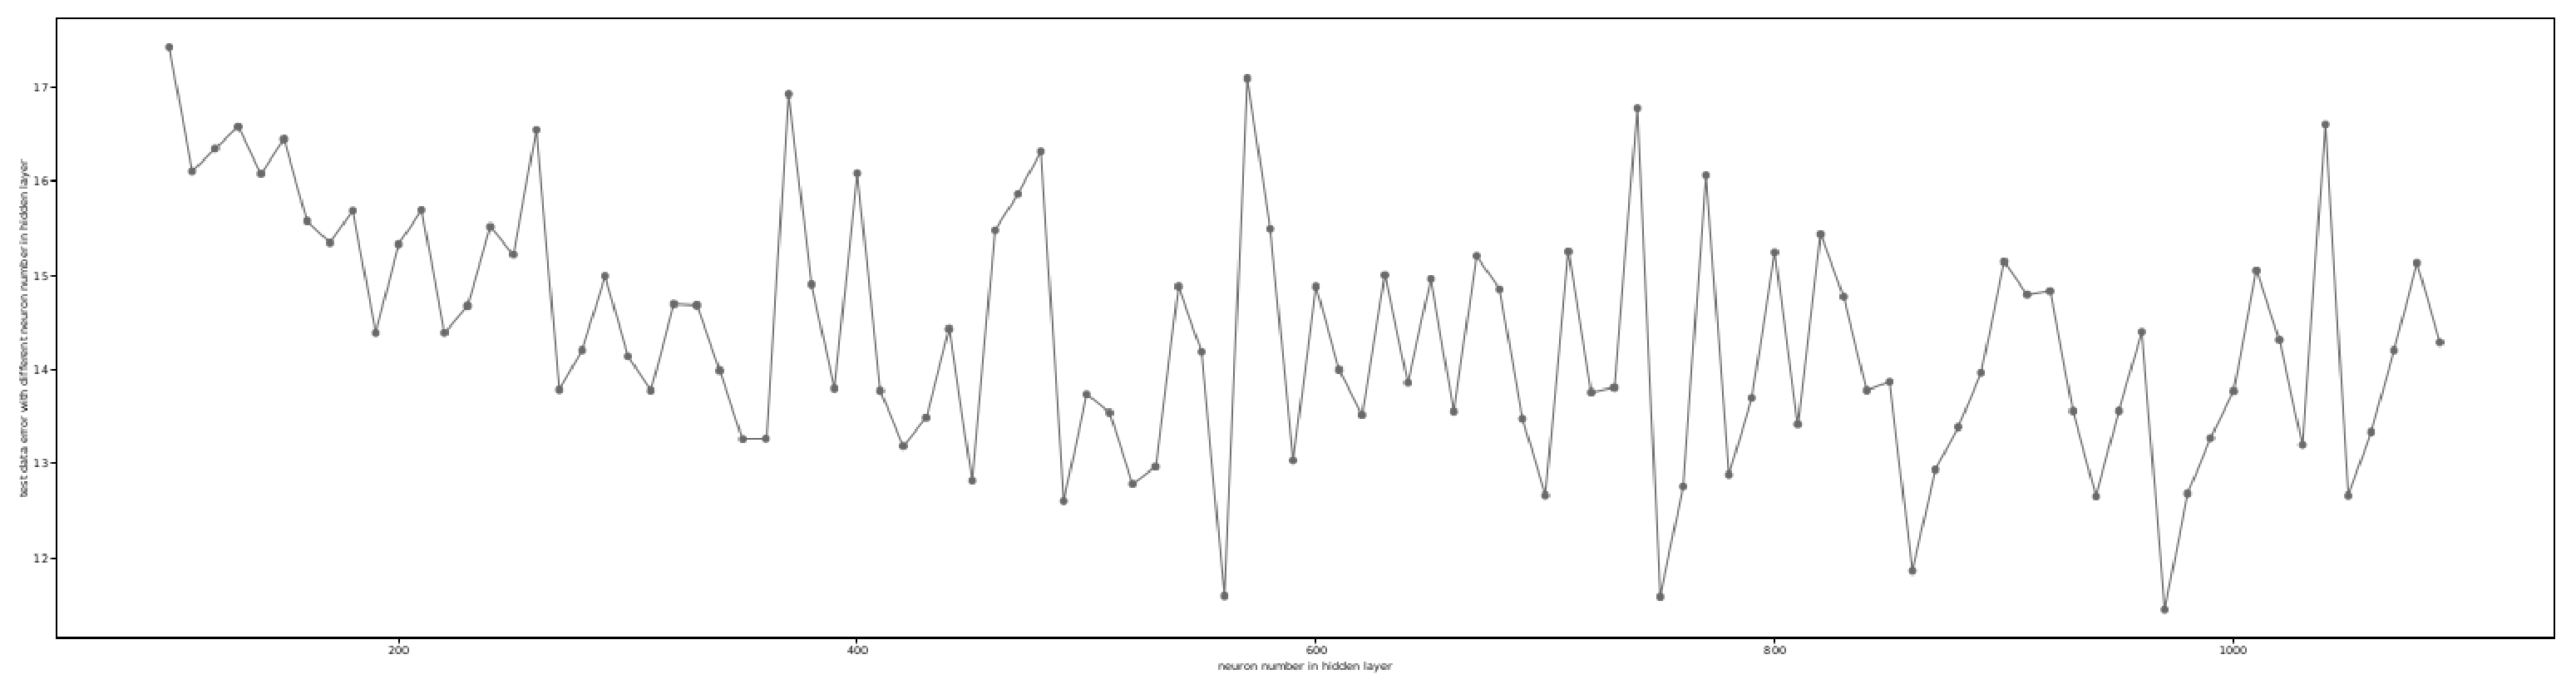
\includegraphics[width=1.0\linewidth]{anti_left.eps}
        \caption{中間層ニューロンの数と左のモーターの出力誤差}
        \label{anti_left}
\end{figure}
\vspace{-5mm}
\begin{figure}[h]
        \centering
        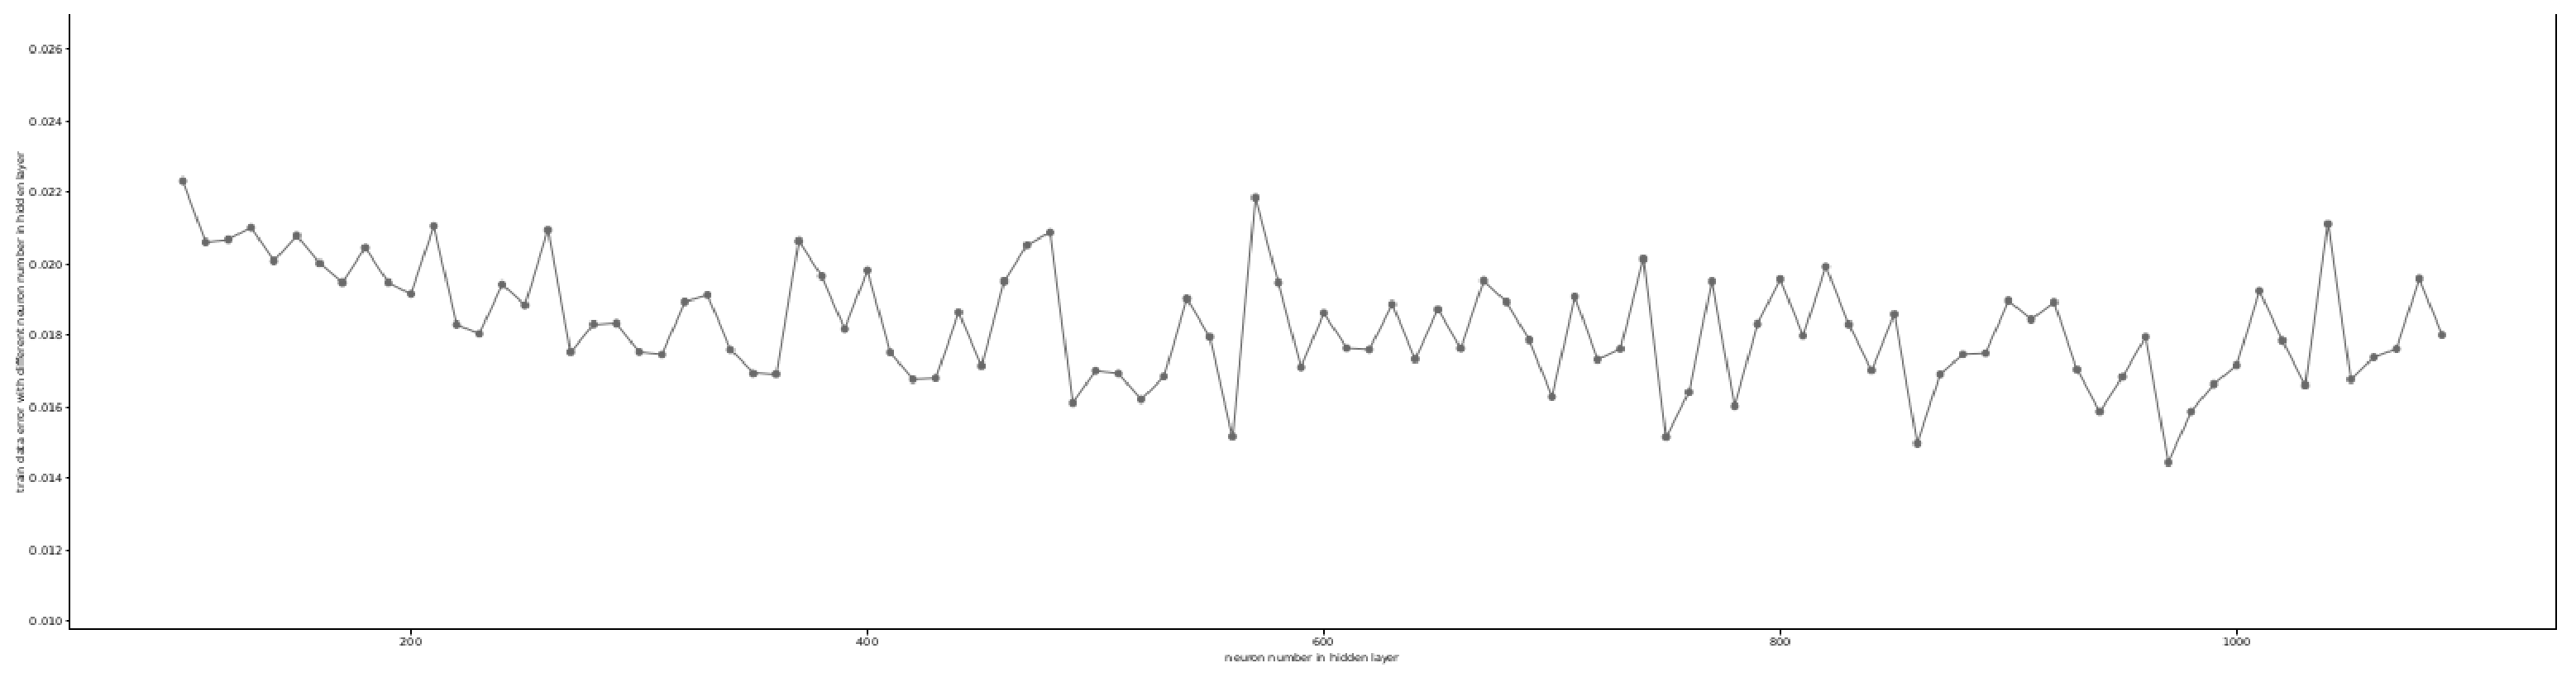
\includegraphics[width=1.0\linewidth]{anti_right.eps}
        \caption{中間層ニューロンの数と右のモーターの出力誤差}
        \label{anti_right}
\end{figure}

\vspace{-7mm}
\begin{figure}[!ht]
    \centering
    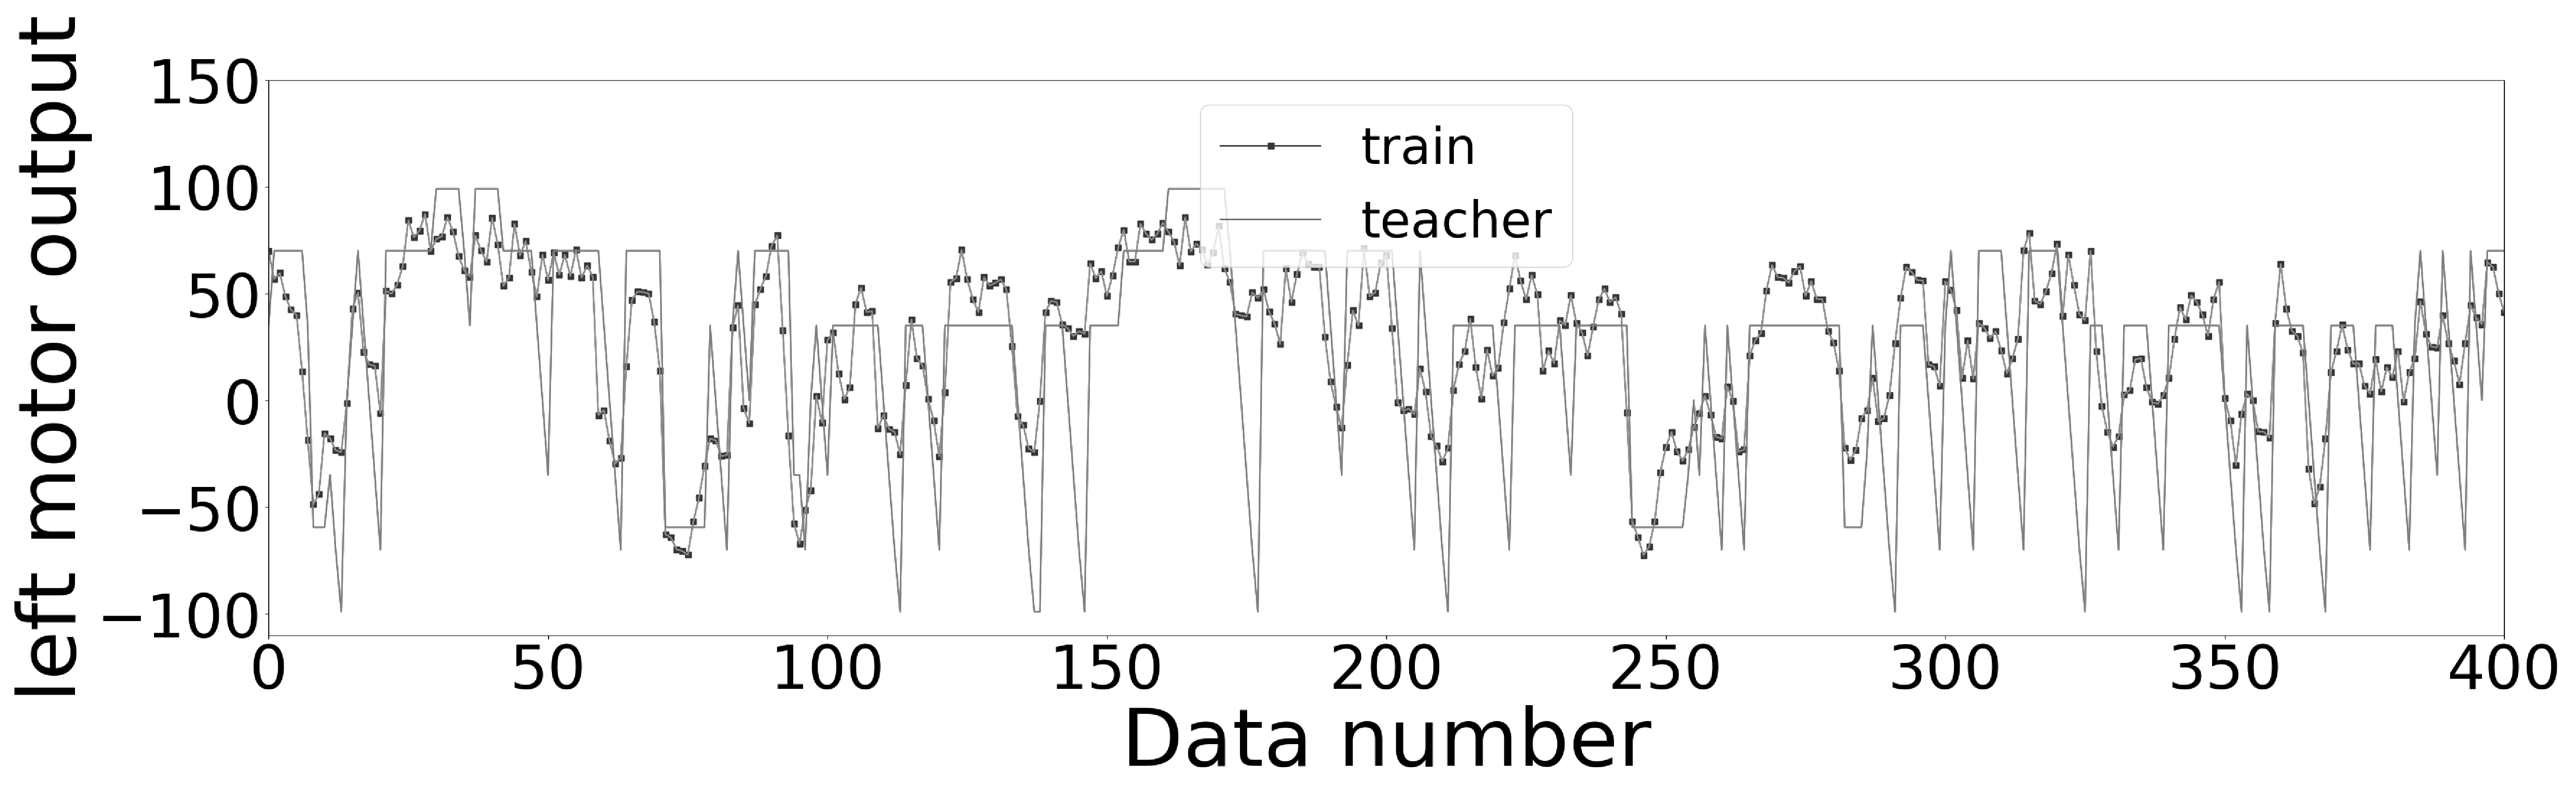
\includegraphics[width=1.0\linewidth]{LeftOutput.eps}
    \caption{NNで左のモーターの出力の回帰結果(局部)}
    \label{LeftOutput}
\end{figure}

\vspace{-7mm}
\begin{figure}[!ht]
    \centering
    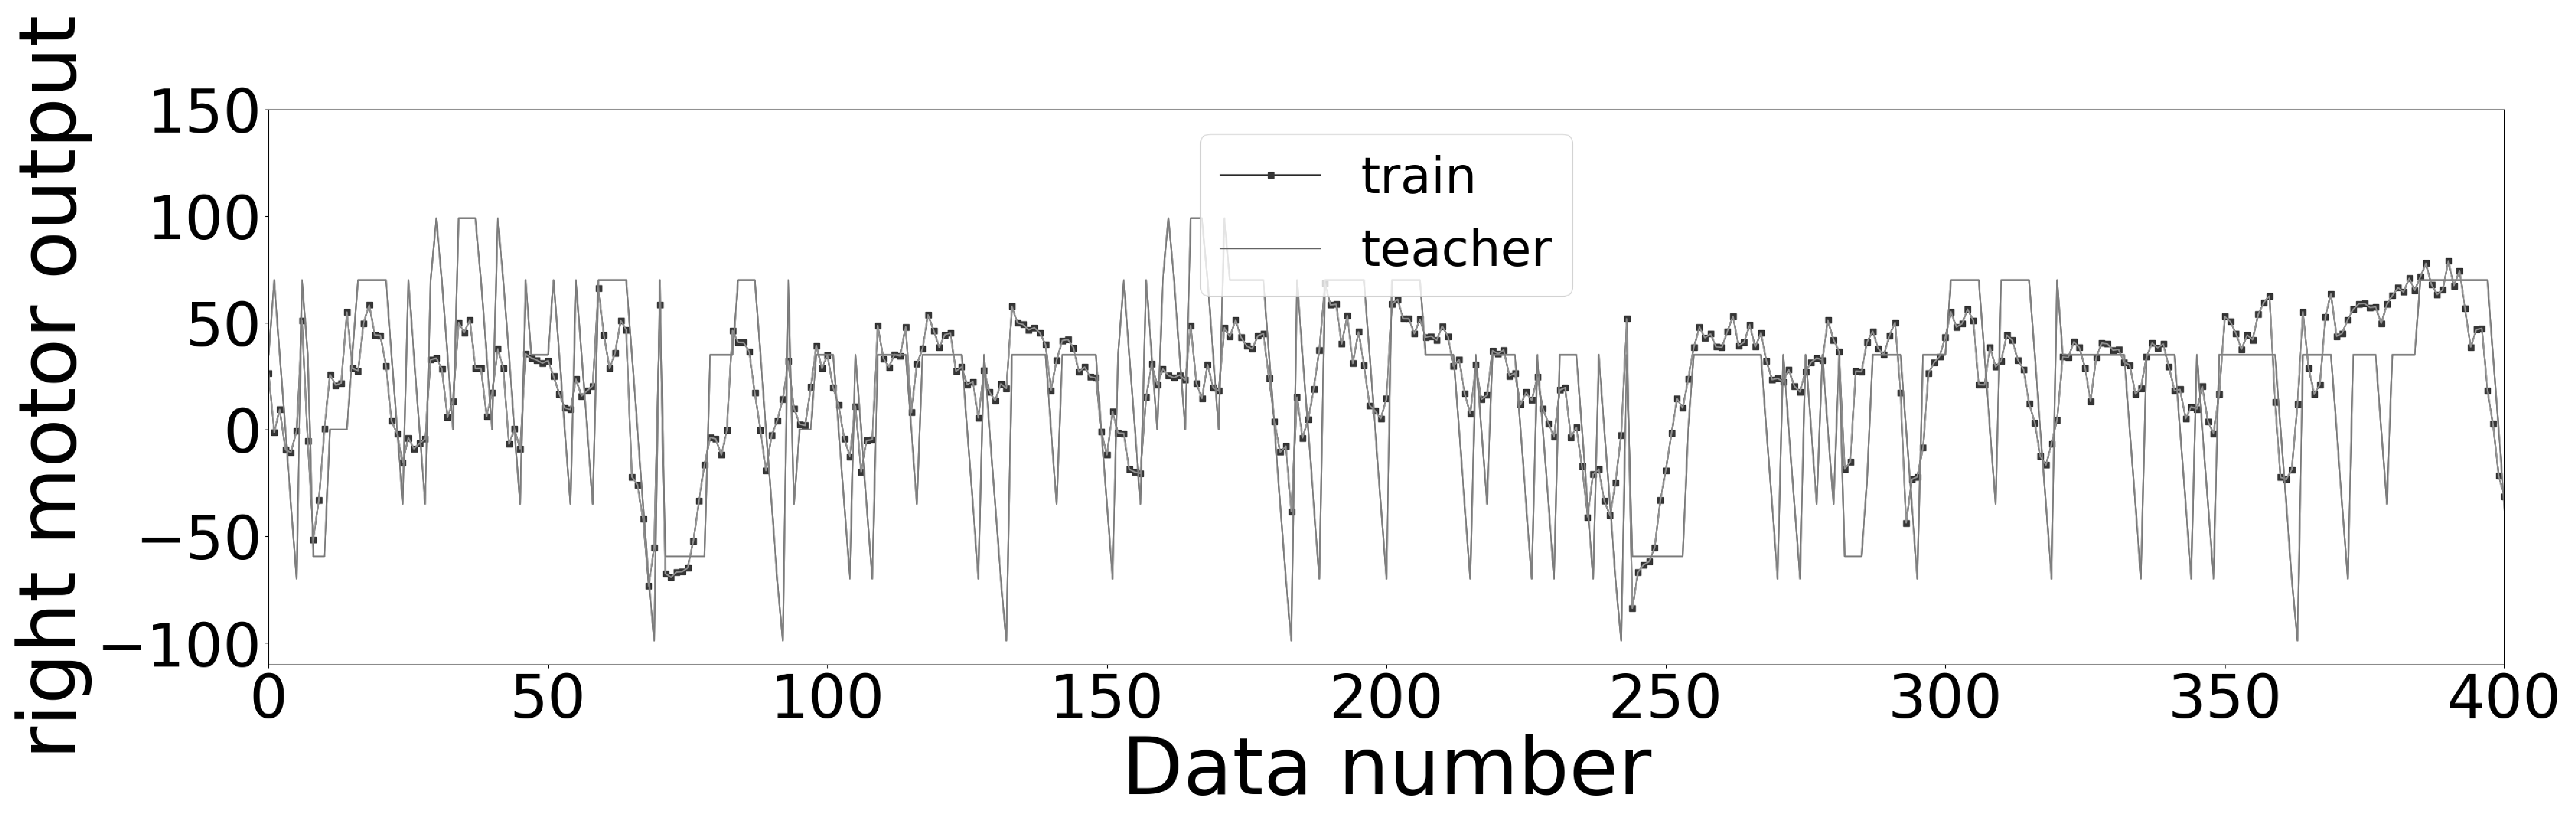
\includegraphics[width=1.0\linewidth]{rightOutput.eps}
    \caption{NNで右のモーターの出力の回帰結果(局部)}
    \label{rightOutput}
\end{figure}

\section{感覚運動写像}
感覚運動写像とは,センサー値を変数とする関数によってモーターの出力を決定することであり,
その瞬間のセンサー値だけを使う,最も単純な反応行動のための知能の一つである\cite{asada}.
本研究では,非線形感覚運動写像モデル(式(\ref{eq:mR})と式(\ref{eq:mL}))が使われている.

3つの距離データを相乗平均する得られた$x_{\rm L}$と$x_{\rm R}$を式(\ref{eq:mR})と
式(\ref{eq:mL})に代入して,ロボットの右モーターの出力($m_{\rm R}$)と左モーターの
出力($m_{\rm L}$)を計算する.
$b$は$\tanh$曲線の変曲点であり,実験ではロボット曲がるの反応距離或いは障害物をぶつからない安全距離である.
今回の実験のパラメーターは
$\alpha=35\%$とする.
すなわちロボットは最高速度の70\%の速度で走行する.ニューラルネットワーク教師データ収集ラジコンする時の最高速度と同じです.
$\beta_1=0.004$,
$\beta_2=10$,
$c=0$とする.
詳しい内容は参考文献\cite{li}を参考してください.

\begin{eqnarray}
\begin{aligned}
  m_{\rm R} = &\alpha \tanh(\beta_1(x_{\rm L} - b_{\rm L})) + \\
        &\alpha \tanh(\beta_2(x_{\rm L} - b_{\rm L})) + c
 \label{eq:mR}
\end{aligned}
\end{eqnarray}

\begin{eqnarray}
\begin{aligned}
  m_{\rm L} = &\alpha \tanh(\beta_1(x_{\rm R} - b_{\rm R})) + \\
        &\alpha \tanh(\beta_2(x_{\rm R} - b_{\rm R})) + c
 \label{eq:mL}
\end{aligned}
\end{eqnarray}

\section{走行実験}
直線とカーブ両方あり,周期境界条件を持ち複数の対面走行できるように,
楕円コースで実験する.
コースの中(青い部分)にロボットをランダムに配置し,半数のロボットが右回り
($b_{\rm L}>b_{\rm R}$),
残りのロボットが左回り($b_{\rm L}<b_{\rm R}$)の向きで,
速度0からほぼ同時にスタート,約8分間実験する.

ロボットがtof距離センサーでコースの障害物までの距離を測って,
非線形感覚運動写像モデルにより走行する.

コースの青い部分の中央(図\ref{fig:cource}黒い線)でコースの長さを測る,
コースの長さ($L$)は7.32$m$,今回ロボットの台数($N$)は8台.
ロボットの線密度 $ \rho = \frac{N}{L} = 1.09 ({\rm 台/m})$

両側の壁を移動させて,コースの幅($w$)を
$43cm$,$49.5cm$,$56cm$,$62.5cm$,$69cm$へ変化させ,実験する.

\begin{eqnarray}
Q_i &=& \frac{|n_i|}{wT_{\rm sd}}
\label{eq:flow} \\
\bar{Q} &=& \frac{1}{N_{\rm exp}}\sum_{i=1}^{N_{\rm exp}} Q_i
\label{eq:flow_ave} 
\end{eqnarray}

\begin{figure}[h]
    \begin{minipage}{0.48\linewidth}
        \centering
        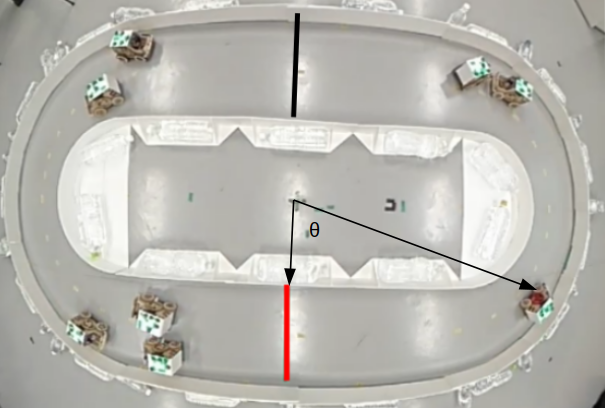
\includegraphics[width=0.9\linewidth]{course3.jpg}
        \caption{実験の様子と$\theta$の説明}
        \label{course1}
    \end{minipage}
    \begin{minipage}{0.48\linewidth}
        \centering
        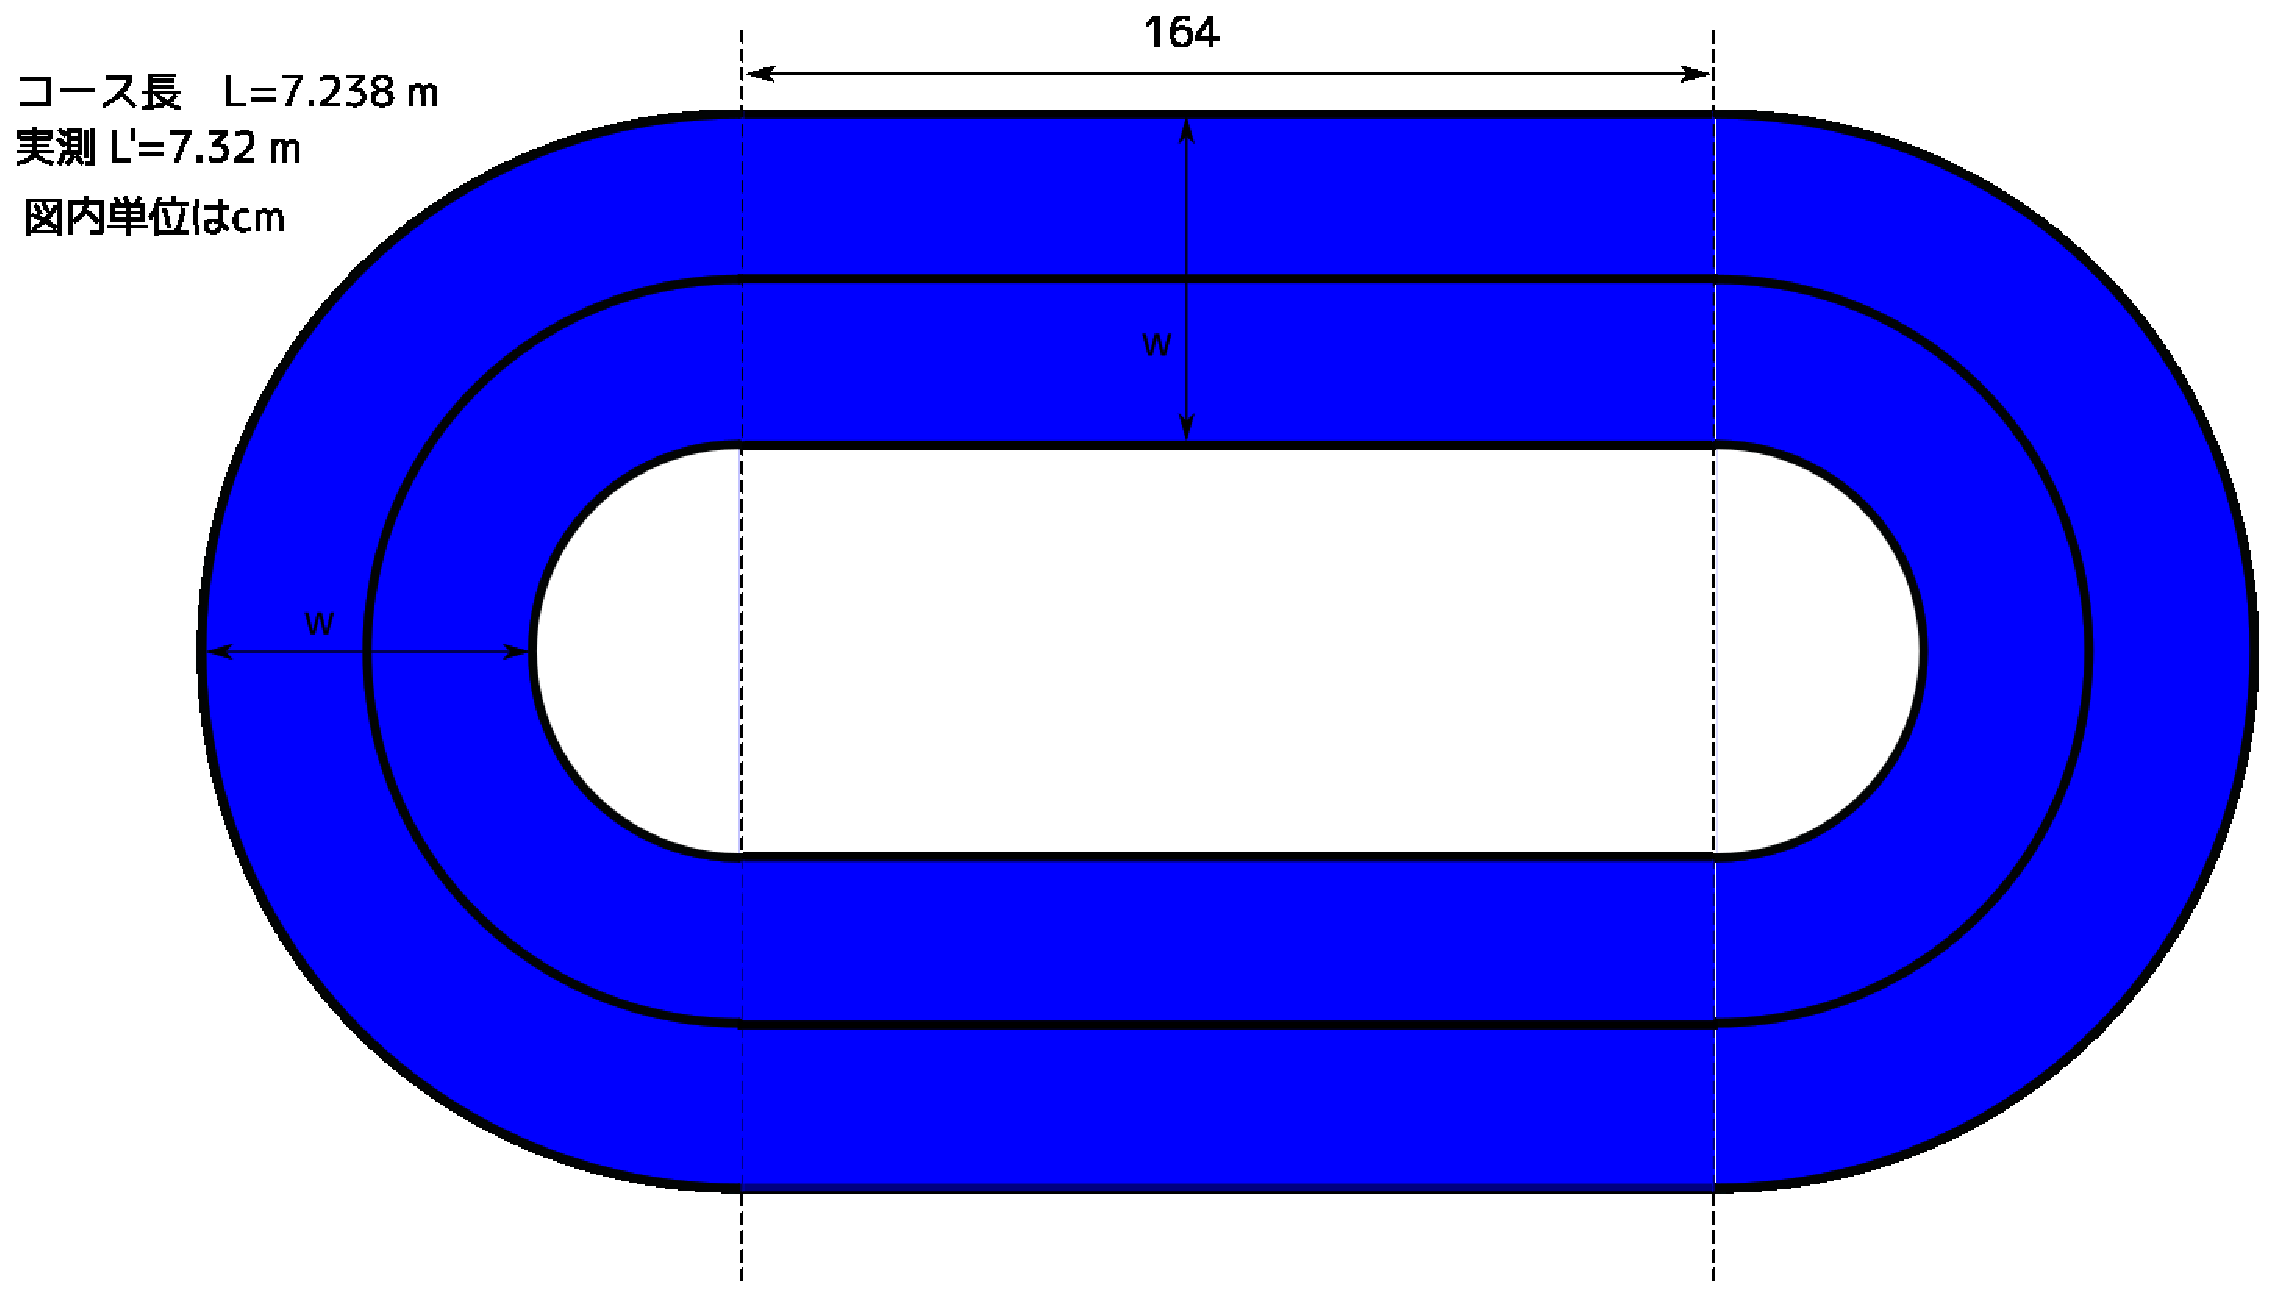
\includegraphics[width=1.0\linewidth]{Oval_h2.eps}
        \caption{\label{fig:cource}コースレイアウト}
        \label{course2}
    \end{minipage}
\end{figure}



図(\ref{course1})の赤い線を計測ラインとして,ロボットが左から右へ線を通過したら流量+1,右から左へ線を通過したら流量-1.図(\ref{course2})の横軸が時間(秒),縦軸がコース中心からみたロボットの位置角度$\theta$(図(\ref{course1})),ロボットが赤い線から反時計回りで黒い線まで,$\theta$が0から$\pi$に変わる.赤い線から時計回りで黒い線まで,$\theta$が0から$-\pi$に変わる.計測ライン(赤い線)を通過して,台数($n$)を計測する.$T_{\rm sd}$はone direction flow 状態になる時間(分),$w$がコースの幅(単位:$m$),$Q$が流量,式(\ref{eq:flow_ave})で流量を計算する.


\section{実験結果}
\subsection{小さいハンドル教師データでの走行}
我々はまず小さいハンドル教師データを学習した結果で,
ランダムの初期配置によって8台ロボット対面走行を実験した.
Fig.\ref{handle15_dia}は時間$s$(横軸)と$\theta$(縦軸上),$R$(縦軸下)の関係図である.
この実験から,一部のロボット達が短時間の対面走行できると確認したが,
ロボット同士がぶつかる,壁にぶつかる,引っかかって解消不能,方向転換なども観察された.
例として,左の上から3番目,右の上から2番目と3番目のグラフで,$\theta$の変動が止まって,水平になった,

\vspace{-1mm}
\begin{figure}[!ht]
    \centering
    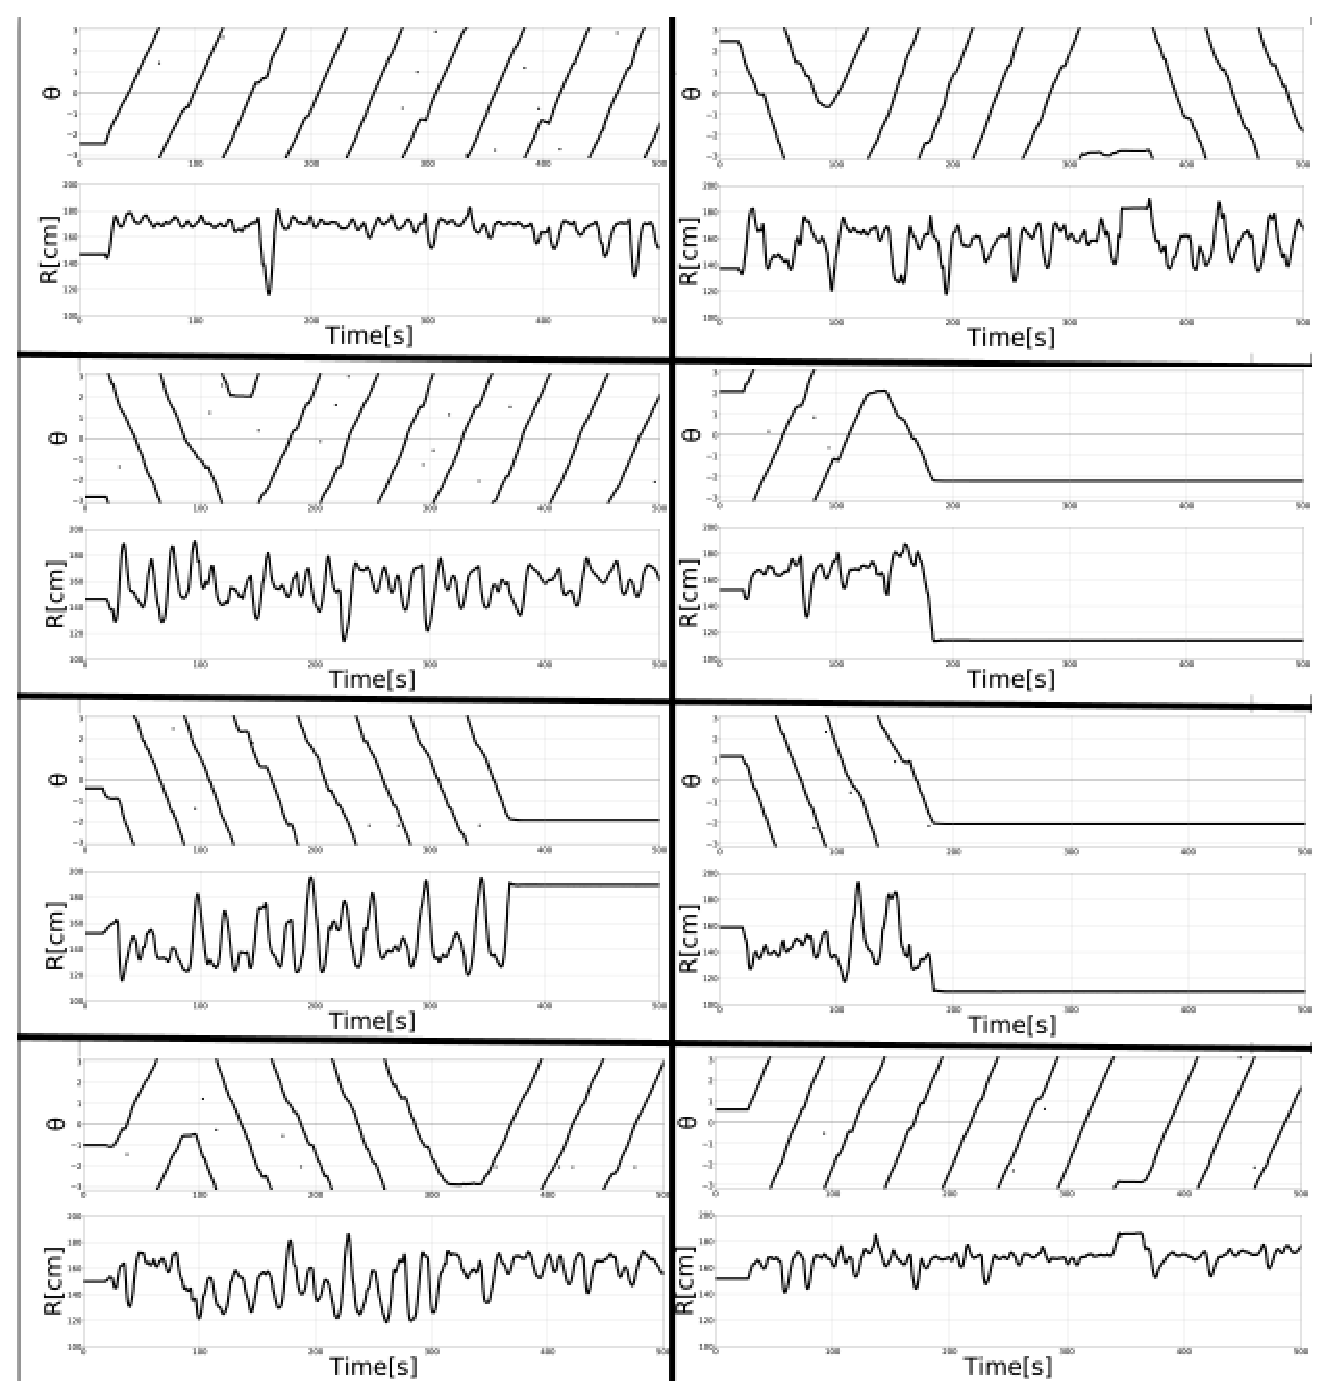
\includegraphics[width=1.0\linewidth]{NN_handle15.eps}
    \caption{小さいハンドル教師データを用いたNNによる8台ロボットの自律走行軌道.
    ロボット同士の膠着状態(図中$\theta,R$の値が一定値になる)が観測された.また方向転換が行われ
    対称的な対面流が崩壊している.}
    \label{handle15_dia}
\end{figure}

Fig.\ref{handle15_img}は約400秒$\theta$が水平になる部分に対する実験風景である.
実験からロボットが壁にぶつかって,後退しなくて停止する.
2つロボットが引っかかって解消不能になって,膠着状態が観察された.
原因として,曲がりと後退のパワーが弱いと考えて,大きいハンドルのラジコンで教師データを
収集して実験した.
実験結果は次に説明する.

\vspace{-5mm}
\begin{figure}[!ht]
    \centering
    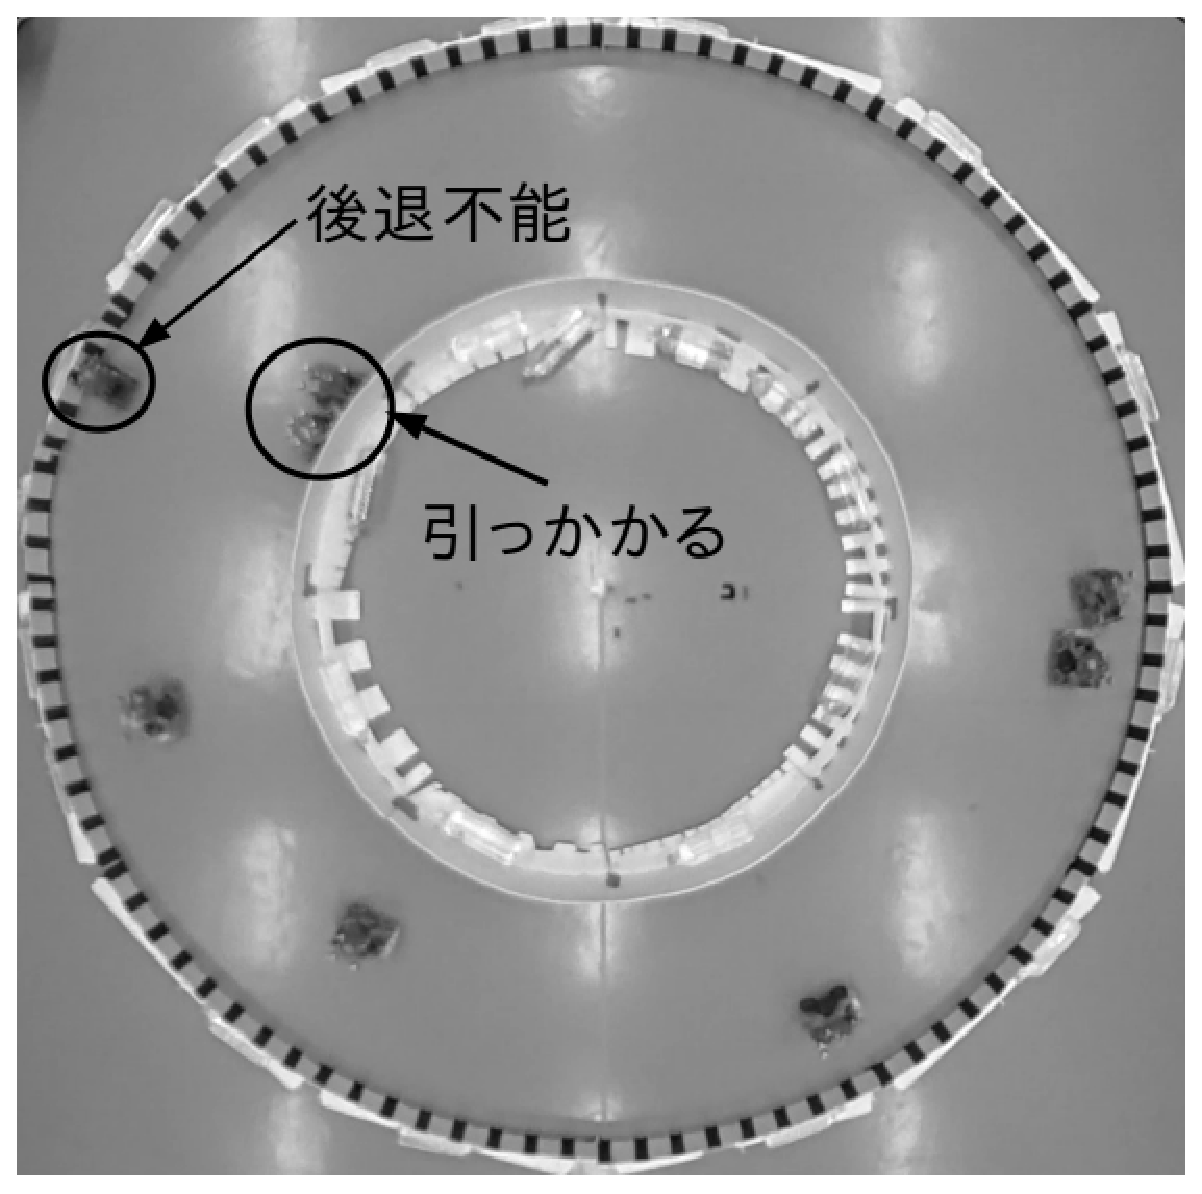
\includegraphics[width=0.6\linewidth]{nnhandle15.eps}
    \caption{小さいハンドルNN走行実験400秒の様子}
    \label{handle15_img}
\end{figure}

\subsection{感覚運動写像と走行の比較}

ラジコンの曲がる値が拡大して(大きいハンドル)収集した教師データの学習結果での自律走行実験も約6回行った.
Fig.\ref{diaRshita}とFig.\ref{diaRshita_270}はニューラルネットワークにより走行と$b=270,270$の感覚運動写像により
走行の1回の走行実験の時間変化におけるロボット位置の角度($\theta$)と半径($R$)のまとめ図である.
横軸は時間(s),縦軸上のほうが$\theta$,下のほうが$R$である.

この2つグラフから,大きいハンドルでのニューラルネットワークよりの走行のほうが対面走行を最後まで維持でき,
スムーズに走れると観察された(Fig.\ref{NN300},時計回りのロボット達が内側の壁に沿う,反時計回りのロボット達が外側の壁に沿う).

$b=270,270$の感覚運動写像によりの走行のほうが途中に1方交流になった(Fig.\ref{diaRshita_270},
約250秒からすべての$theta$の曲線が右に傾斜する),
$R$の変動範囲が大きい(衝突が多い),1方向走行流になったら,$R$の変動も安定になって,
外側の壁に沿って反時計回り走ると観察された(Fig.\ref{SMM300}).


\vspace{-1mm}
\begin{figure}[!ht]
    \centering
    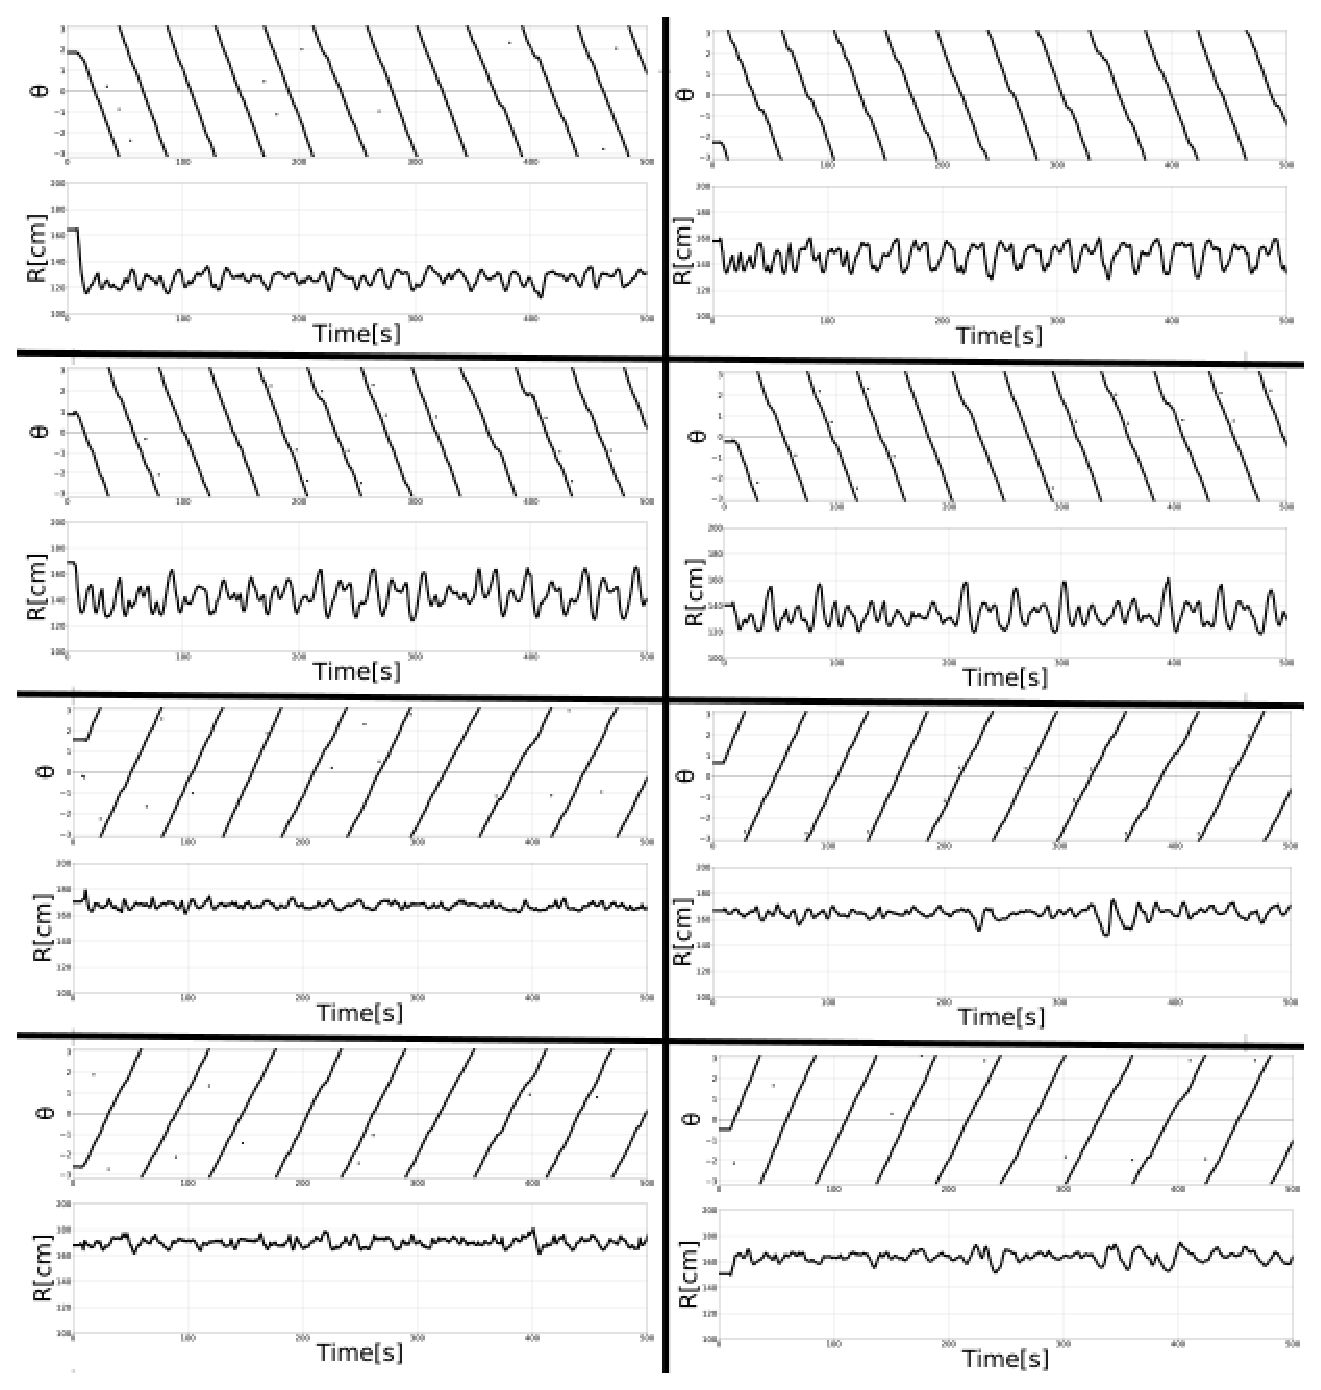
\includegraphics[width=1.0\linewidth]{nn_shita_R_rand.eps}
    \caption{ランダムの初期配置でNNにより走行の$\theta$,$R$と時間の関係図}
    \label{diaRshita}
\end{figure}

\vspace{-4mm}
\begin{figure}[!ht]
    \centering
    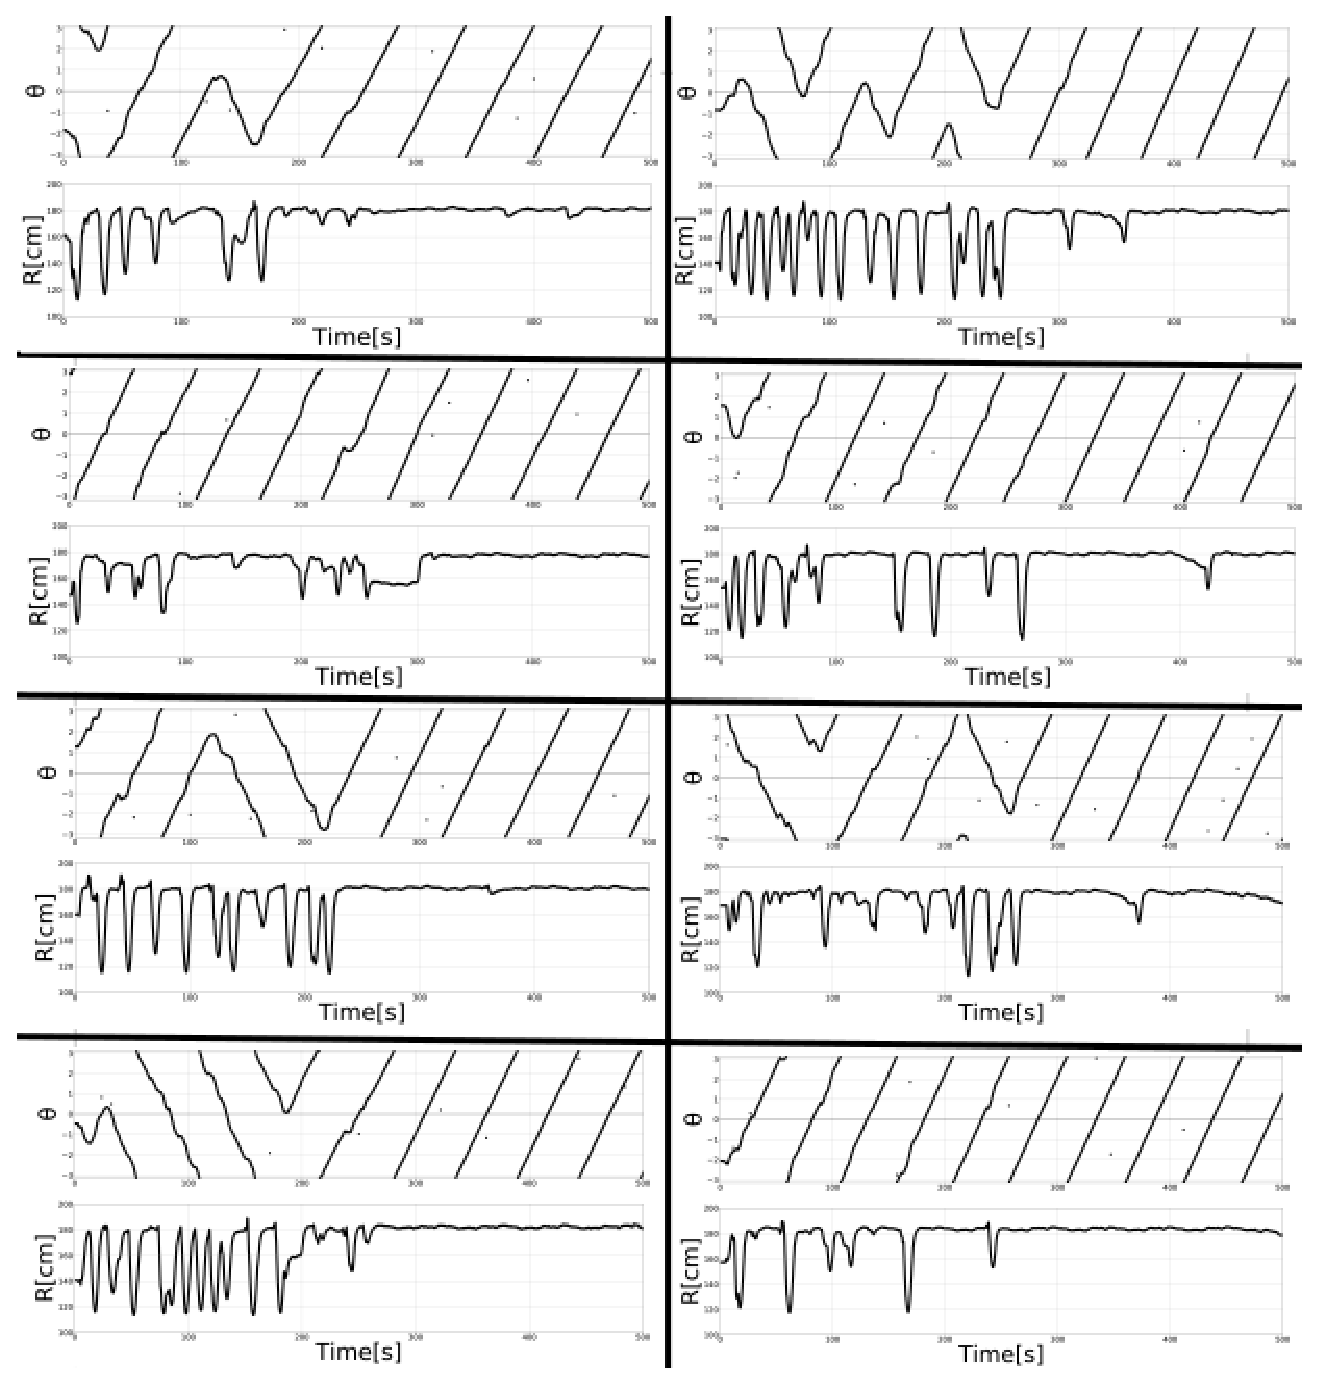
\includegraphics[width=1.0\linewidth]{smm_shita_R_rand270.eps}
    \caption{ランダムの初期配置でSMMにより走行の$\theta$,$R$と時間の関係図}
    \label{diaRshita_270}
\end{figure}

\begin{figure}[h]
    \begin{minipage}{0.48\linewidth}
        \centering
        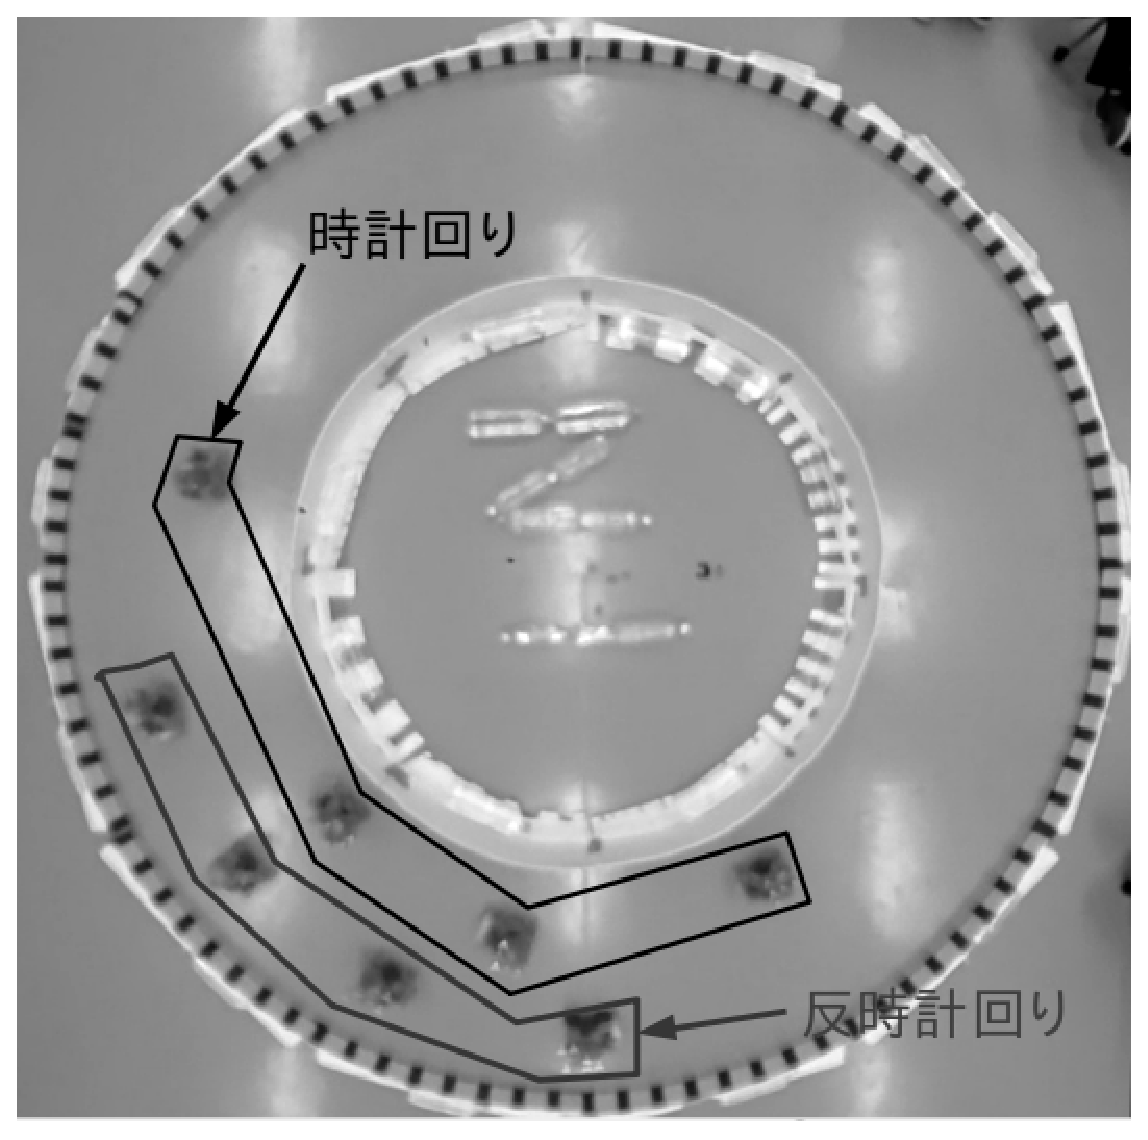
\includegraphics[width=1.0\linewidth]{NN_exp.eps}
        \caption{300秒neural network走行風景}
        \label{NN300}
    \end{minipage}
    \begin{minipage}{0.48\linewidth}
        \centering
        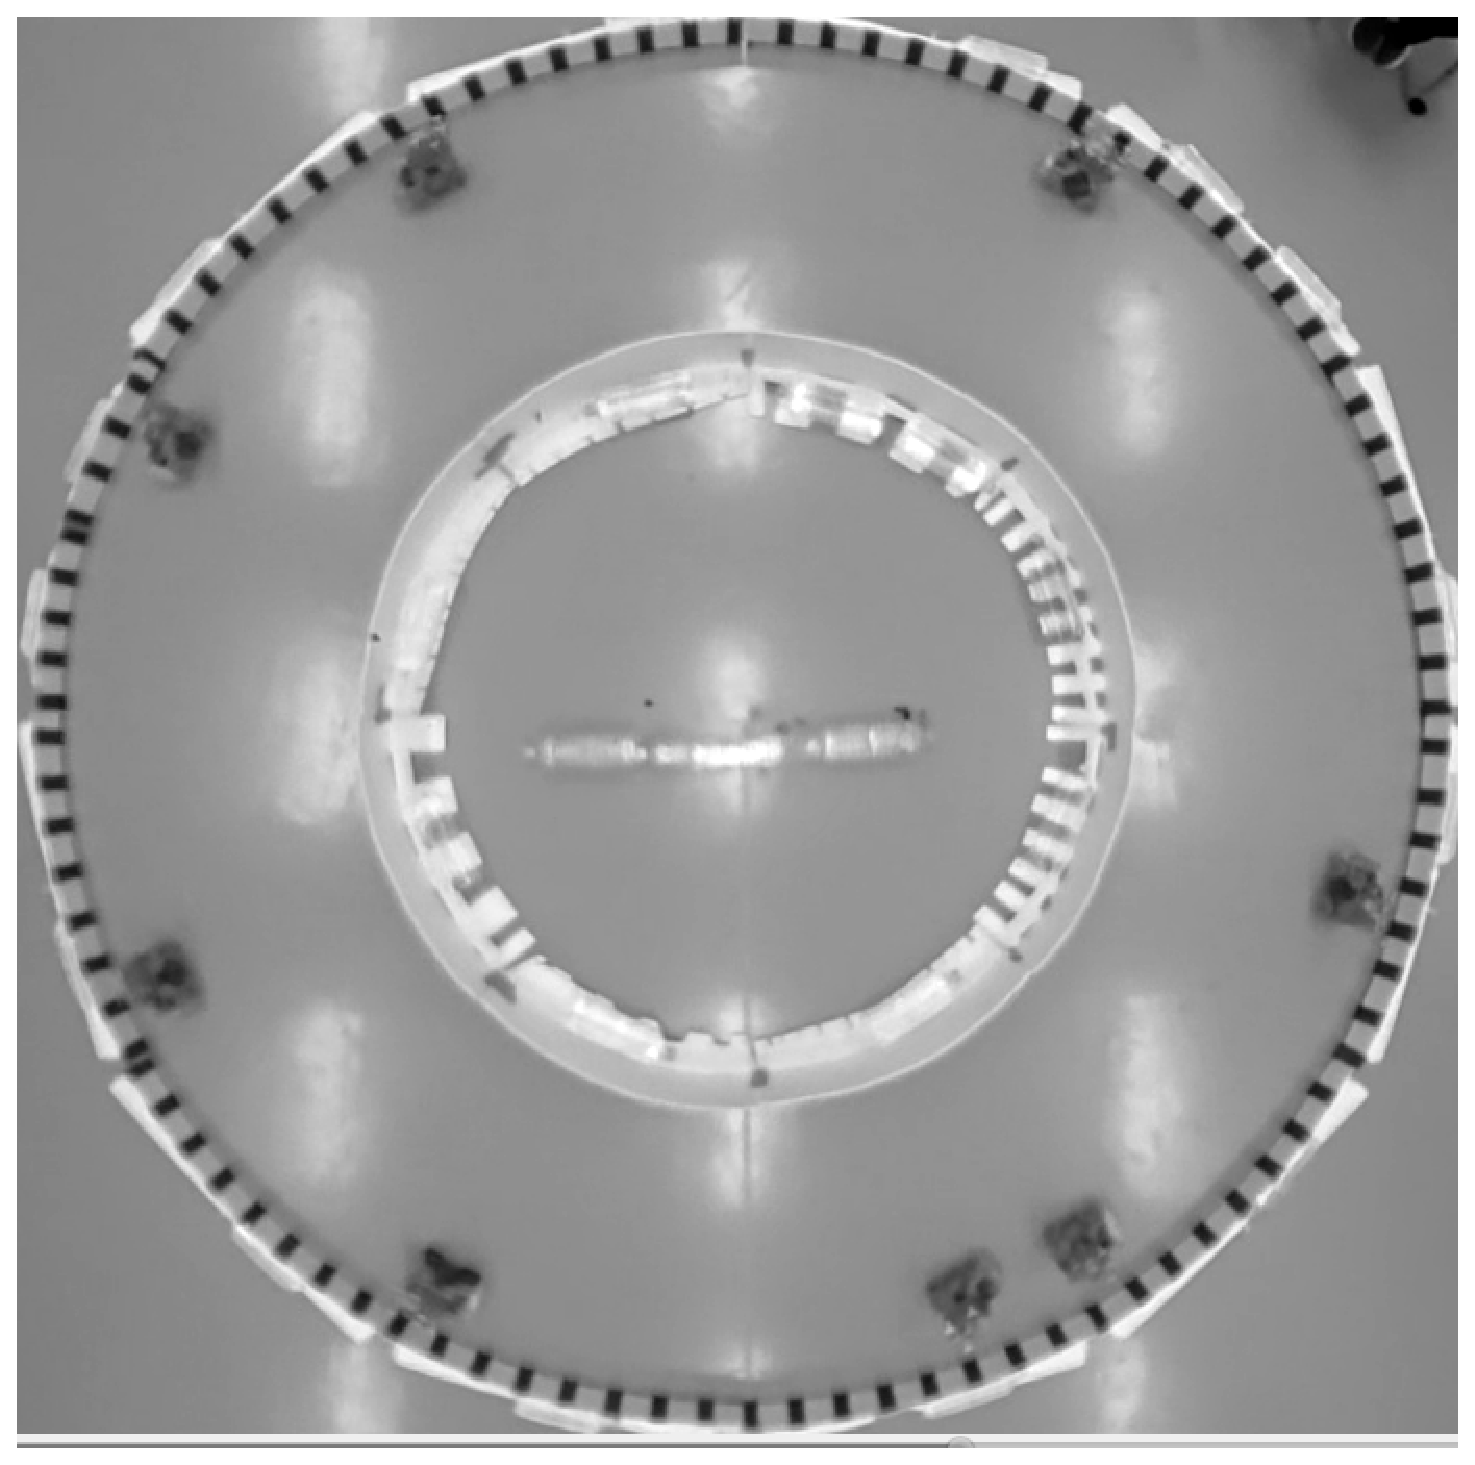
\includegraphics[width=1.0\linewidth]{SMM270_exp.eps}
        \caption{300秒感覚運動写像走行風景}
        \label{SMM300}
    \end{minipage}
\end{figure}

\subsection{感覚運動写像と流量の比較}
流量を比較するため,ランダムと渋滞,2種類の初期配置でニューラルネットワークより,感覚運動写像より約5回実験した.
Fig.\ref{random_result}とFig.\ref{crowd_result}は2種類の初期配置での実験回数($x$軸)と流量($y$軸)の関係図です.

点線がニューラルネットワークより走行の結果,実線が$b=270,270$の感覚運動写像より走行の結果,一点鎖線が$b=360,260$の感覚運動写像より走行の結果です.
ニューラルネットワークの流量が常に感覚運動写像の流量より高い,変動も平穏だと見られる.

Fig.\ref{compare_result}はランダムの初期配置(実線)と渋滞の初期配置(一点鎖線)で約5回の実験の流量平均値グラフです.
$x$軸はアルゴリズム種類,$y$軸は平均流量.この図からニューラルネットワークの平均流量も感覚運動写像より高くて,異なる初期配置に対して平均流量があんまり変わらない.
$b=270,270$の感覚運動写像の平均流量が初期配置によって差が観察されて,それは実験の回数が不足かなと考えて,今後,実験の回数を増やす必要があると思う.


\vspace{-1mm}
\begin{figure}[!ht]
    \centering
    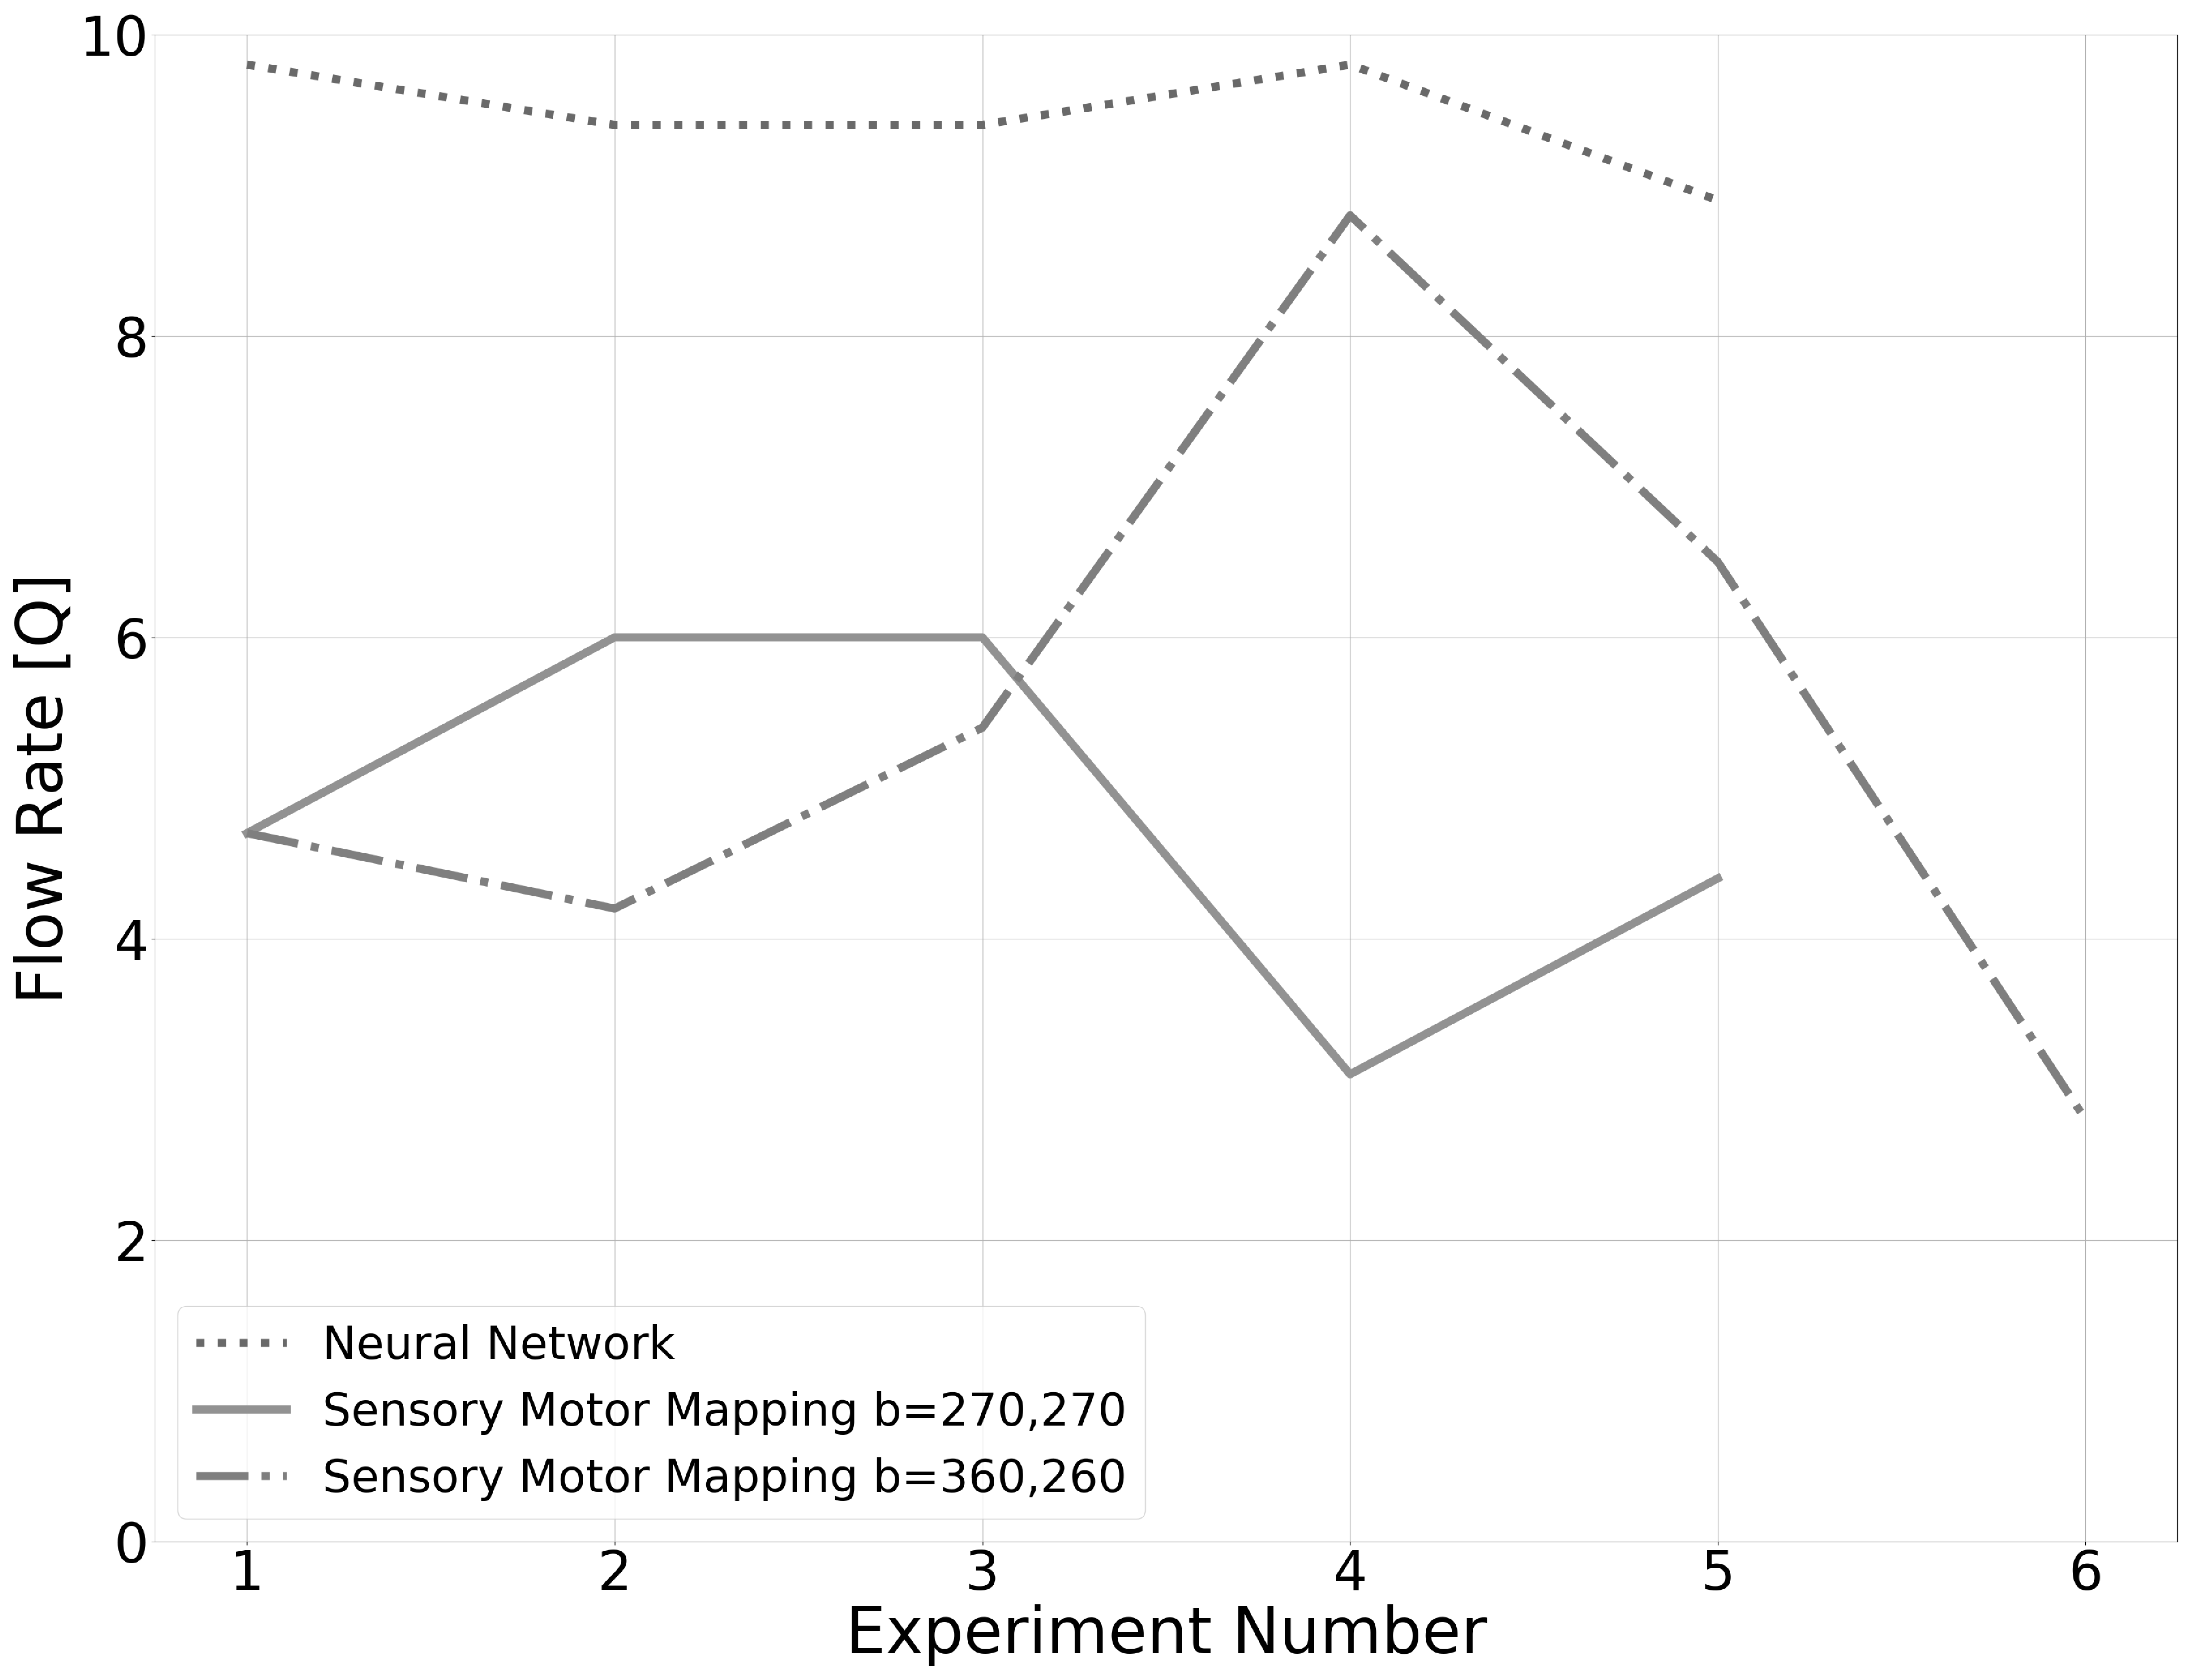
\includegraphics[width=0.9\linewidth]{result_diagrim_rand.eps}
    \caption{ランダムの初期配置で実験回数により流量の変化図}
    \label{random_result}
\end{figure}


\vspace{-1mm}
\begin{figure}[!ht]
    \centering
    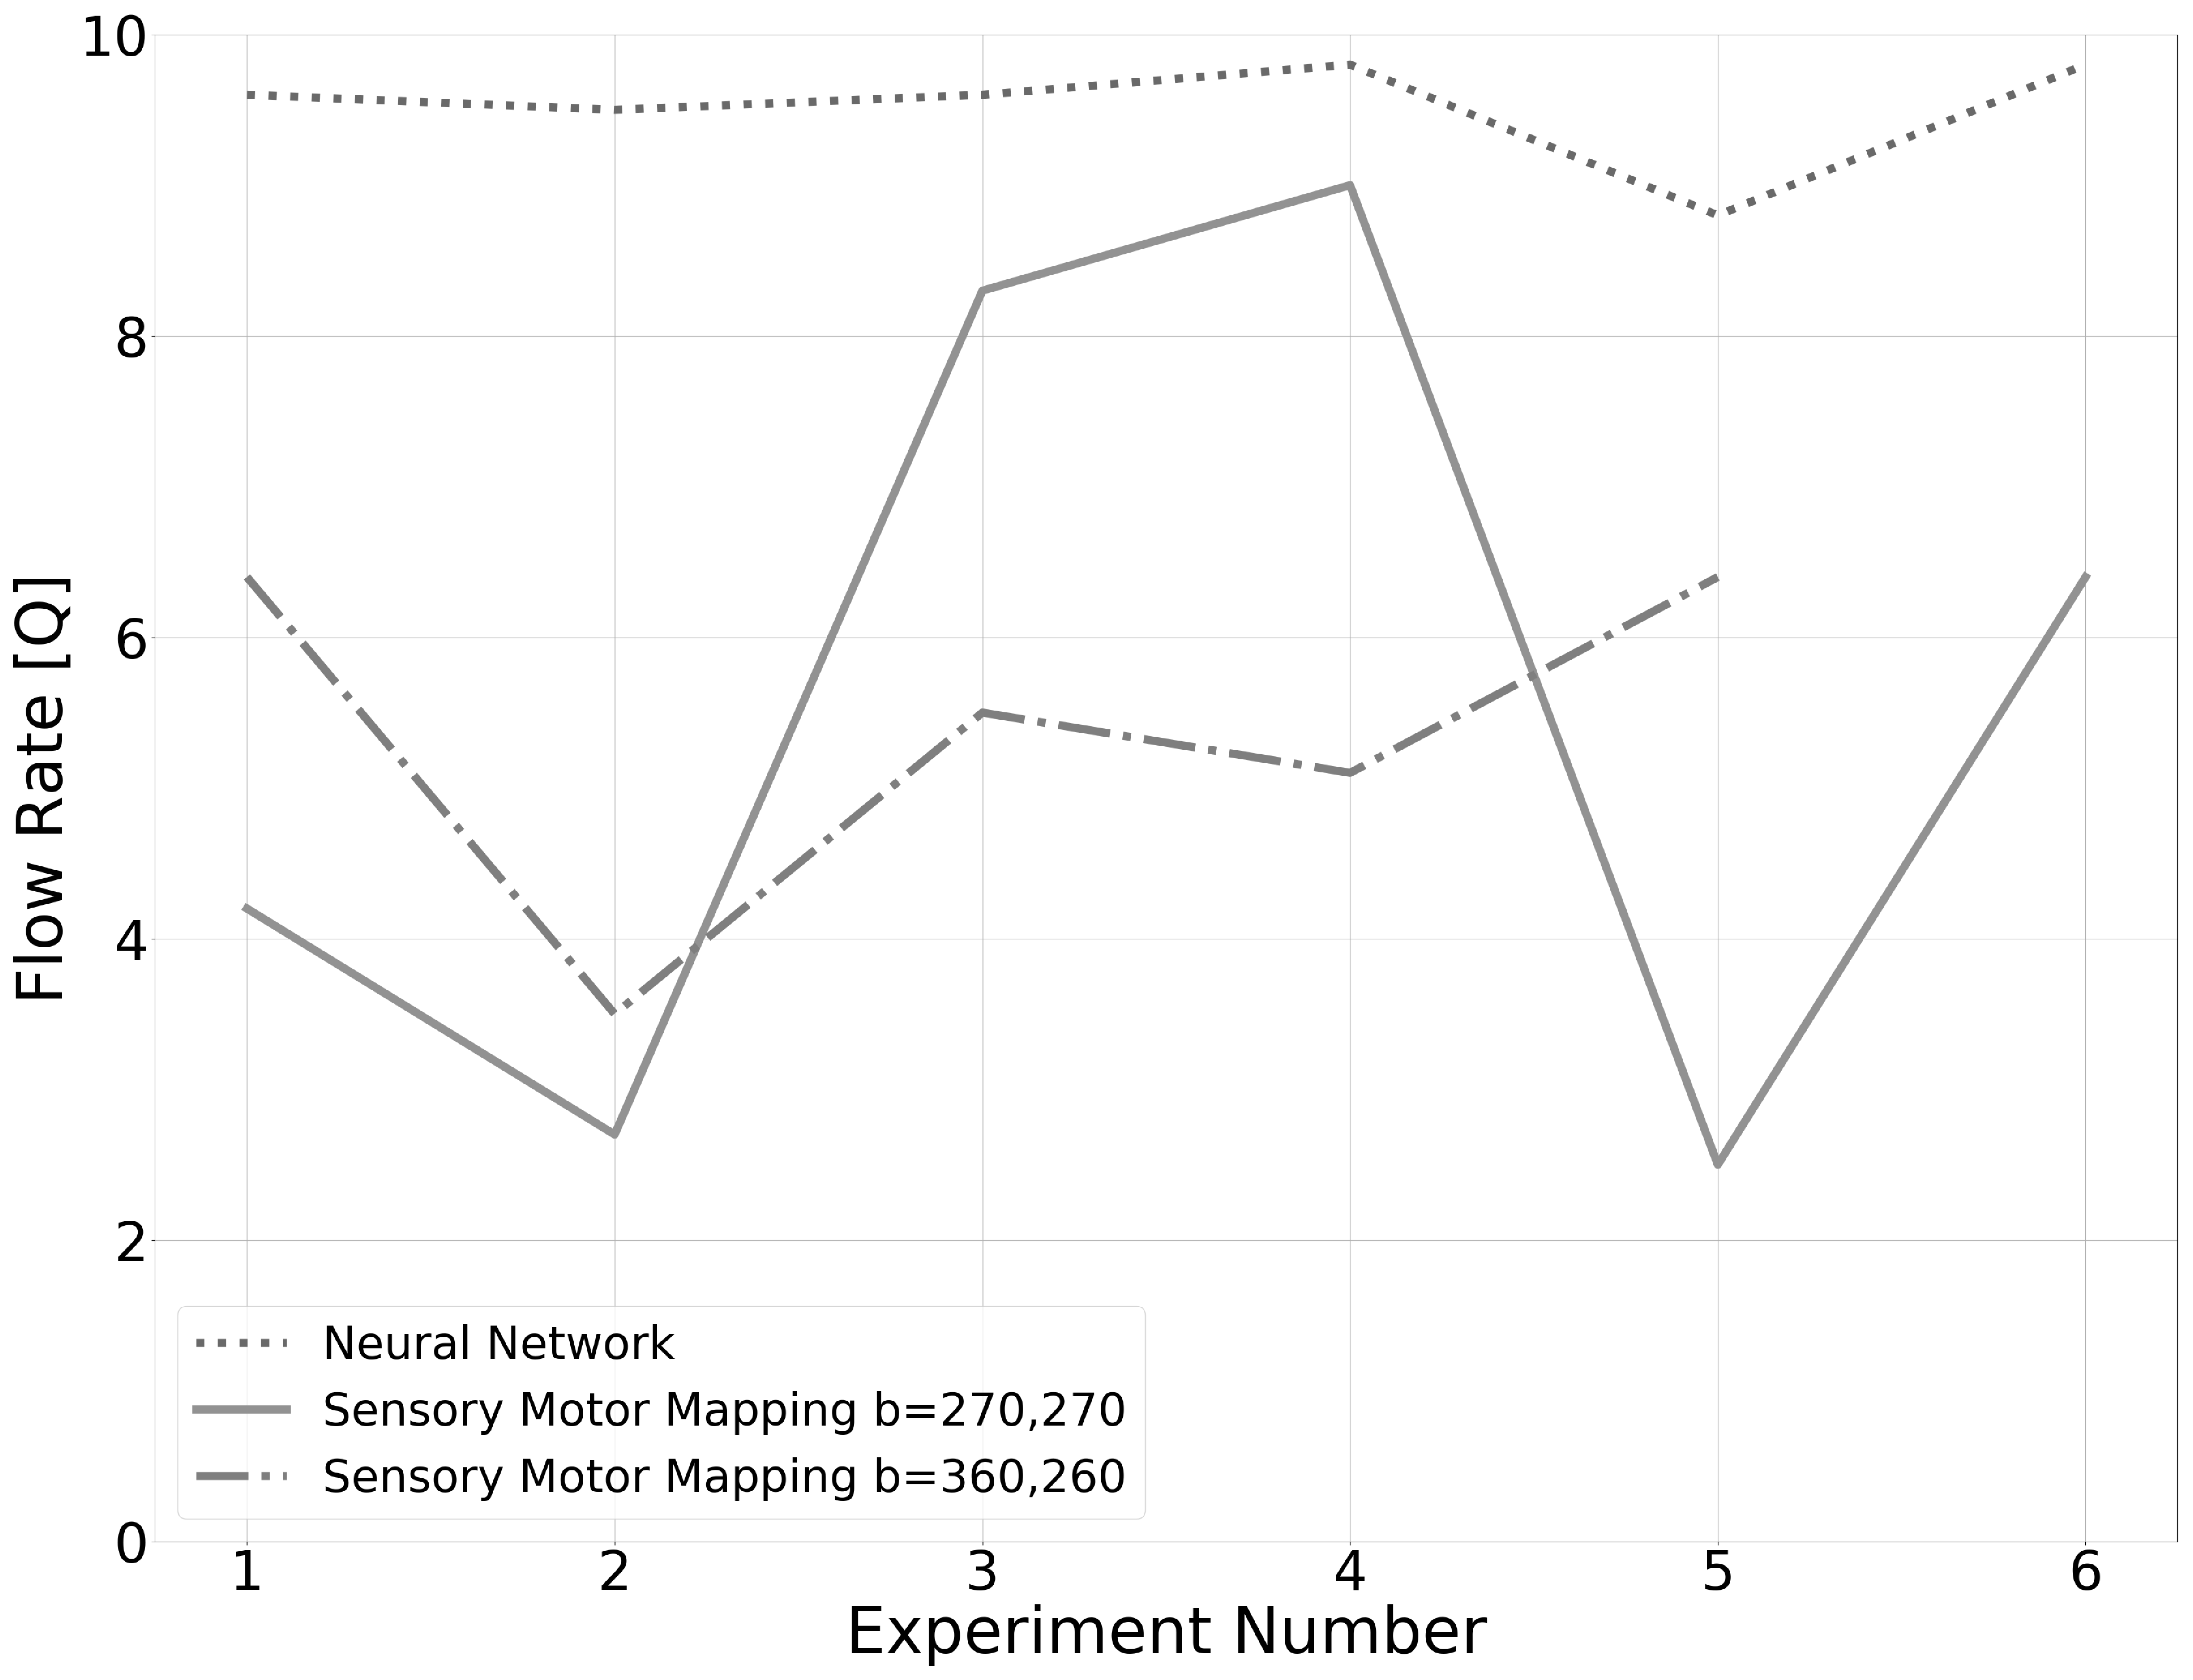
\includegraphics[width=0.9\linewidth]{result_diagrim_crow.eps}
    \caption{渋滞の初期配置で実験回数により流量の変化図}
    \label{crowd_result}
\end{figure}


\vspace{-1mm}
\begin{figure}[!ht]
    \centering
    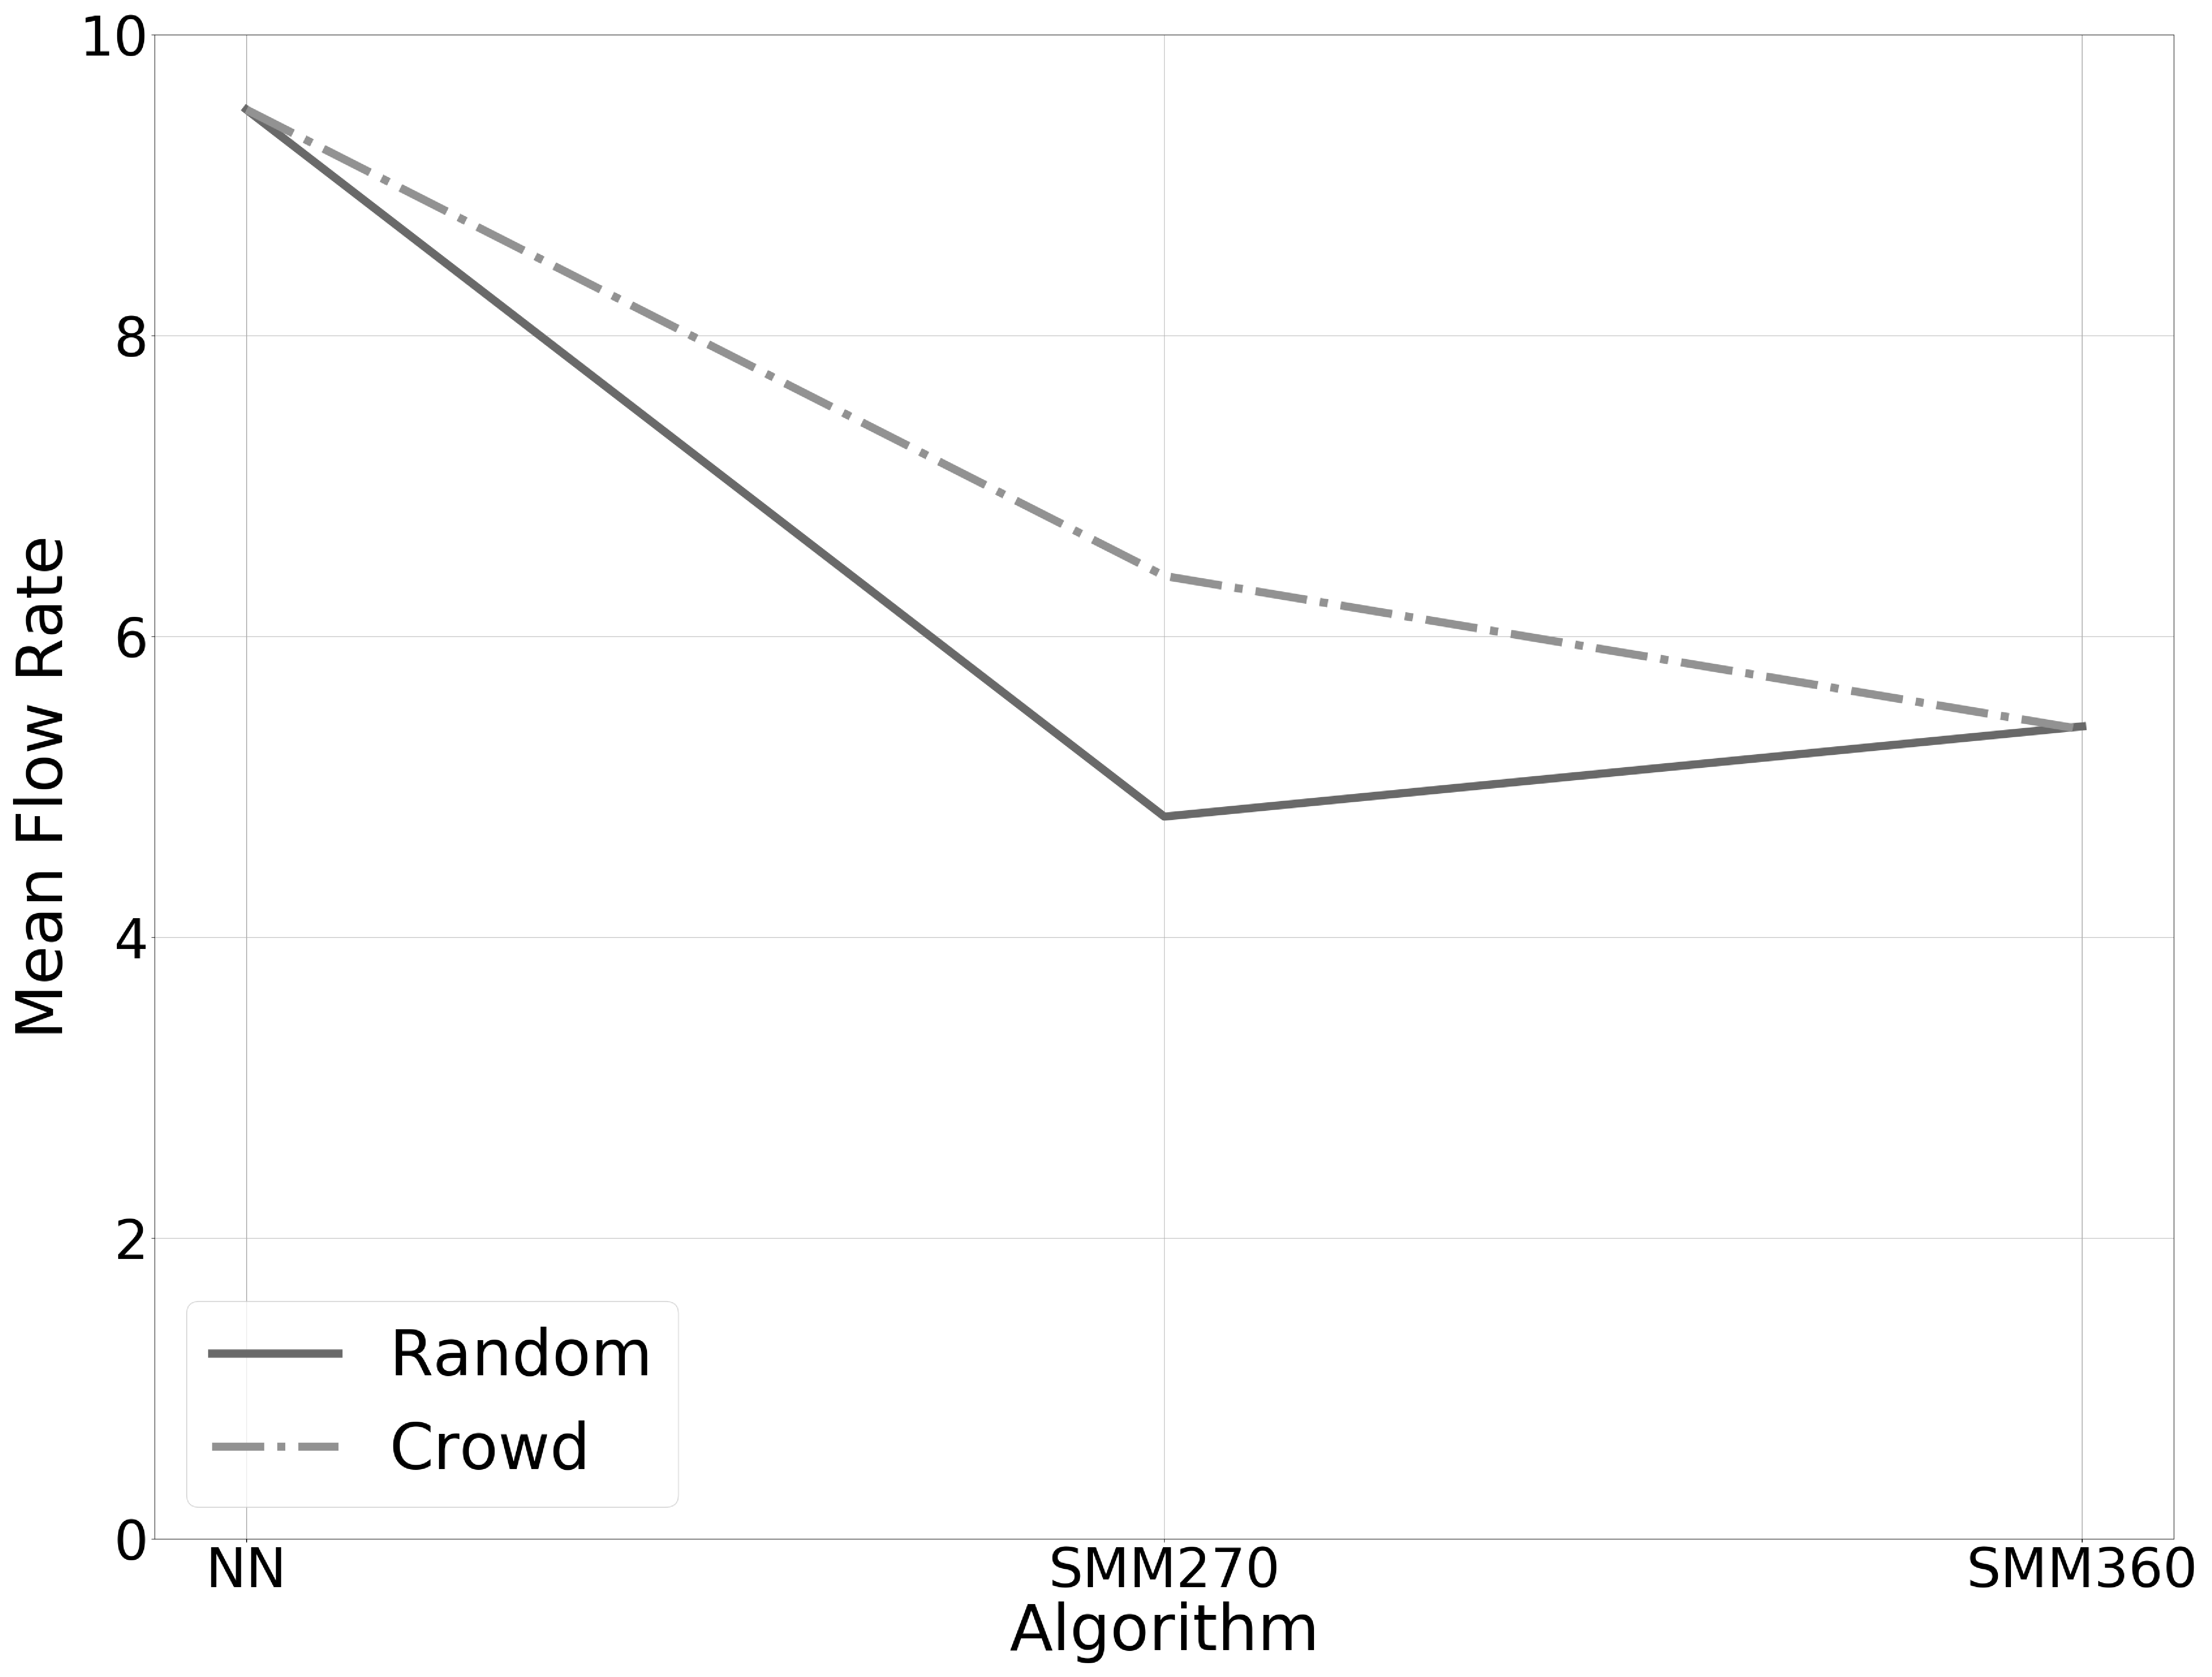
\includegraphics[width=0.9\linewidth]{mean_Q.eps}
    \caption{異なるアルゴリズムの平均流量の比較}
    \label{compare_result}
\end{figure}

\section{まとめ}
1次元画像データ認識ニューラルネットワークより8台ロボットが縞模様のコースで対面走行ができると確認した.
感覚運動写像と比べて,方向転換教えなくても,対面走行を維持する能力が高い.

本文説明した対面走行維持できるニューラルネットワークの学習結果は,著者が何十回練習して,経験を踏まえ,ラジコンする時,遠くから曲がる,近づいて曲がる,真正面にロボットや壁ある時後退することをわざわざ人間の意識持ってロボットに教えて収集した教師データの学習結果です,研究室の他の人がラジコンして収集した教師データも学習して,自律走行の質もそれぞれだ.それに,コースの壁の代わりに,別のもの(ダンボール,雑誌,サンダルなど)を配置して,収集した教師データの学習結果では自律走行ができないことが観察された,その原因として,画像を列ずつ足し算してもらった1次元画像データが障害物と通路の特徴を失って,区別できなくなると考える.

今後の展望として,色んな教師データの違いと特徴をを分析して,どんな教師データがあれば対面走行維持できるを解明すると教師データの質を評価方法を開発する必要がある.
また,画像エントロピーで環境の複雑度を評価して1次元画像データの限界を解明すると考える.


\begin{thebibliography}{9}
\bibitem{murakami2021}H.Murakami, C.Feliciani, Y.Nishiyama and K. Nishinari,
"Mutual anticipation can contribute to self-organization in human crowds" 
Vol 7 Issue 12 Science Advances (2021).
\bibitem{li2020} 李 方 正, 橋爪晋平, 本田泰.「非線形感覚運動写像ロボットの対面流–1 方向走行流への転移と流量のコース幅依存性–」第26回交通流と自己駆動粒子系シンポジウム論文集 (2020)
\bibitem{asada} 浅田稔,国吉康夫「ロボットインテリジンス」(2006).
\end{thebibliography}
\end{document}
